\documentclass{article}

\PassOptionsToPackage{numbers,compress}{natbib}

% Creative AI Track (matches the Call for Creative AI, NeurIPS 2026).
% At submission time this stays anonymous with line numbers.
\usepackage[creativeai]{neurips_2026}
% For a camera-ready version, use: \usepackage[creativeai, final]{neurips_2026}
% For an arXiv preprint, use:      \usepackage[preprint]{neurips_2026}


\usepackage[utf8]{inputenc} % allow utf-8 input
\usepackage[T1]{fontenc}    % use 8-bit T1 fonts
\usepackage{hyperref}       % hyperlinks
\usepackage{url}            % simple URL typesetting
\usepackage{booktabs}       % professional-quality tables
\usepackage{tabularx}       % width-constrained wrapping tables
\usepackage{amsfonts}       % blackboard math symbols
\usepackage{amsmath}
\usepackage{nicefrac}       % compact symbols for 1/2, etc.
\usepackage{microtype}      % microtypography
\usepackage{xcolor}         % colors
\usepackage{graphicx}
\usepackage[font=small,labelfont=bf,skip=3.5pt]{caption}
\usepackage{subcaption}
\usepackage{enumitem}      % compact contribution bullets
\usepackage{tikz}
\usetikzlibrary{arrows.meta, positioning, shapes.geometric, calc, backgrounds, fit}
\usepackage[most]{tcolorbox}

% Boxes for prompts / persona reactions / edit instructions (supplement).
\newtcolorbox{promptbox}[1]{colback=black!5, colframe=black!80, coltitle=white,
  colbacktitle=black!80, fonttitle=\bfseries\small, title={#1}, boxrule=0.6pt, arc=2pt,
  left=5pt, right=5pt, top=3pt, bottom=3pt, breakable}
\newtcolorbox{personabox}[1]{colback=black!4, colframe=black!45, coltitle=black,
  colbacktitle=black!12, fonttitle=\bfseries\footnotesize, title={#1}, boxrule=0.5pt, arc=2pt,
  left=5pt, right=5pt, top=2pt, bottom=2pt}
\newtcolorbox{instrbox}[1]{colback=black!5, colframe=black!80, coltitle=white,
  colbacktitle=black!80, fonttitle=\bfseries\small, title={#1}, boxrule=0.6pt, arc=2pt,
  left=5pt, right=5pt, top=3pt, bottom=3pt}
% typewriter prompt text: straight quotes and real hyphens (no ligatures)
\newcommand{\pt}[1]{{\ttfamily\footnotesize #1}}

% Palette shared with all figures (validated categorical hues).
\definecolor{aeblue}{HTML}{2A78D6}   % primary  — synthetic audience
\definecolor{aegreen}{HTML}{1BAF7A}  % tertiary — editing loop
\definecolor{aered}{HTML}{EB6834}    % secondary — held-out judge
\definecolor{aegray}{HTML}{8A8A86}
\definecolor{aelight}{HTML}{E7F0FB}
\definecolor{aelightg}{HTML}{E4F5EE}

% Model-provider marks used as corner badges in Figure 1 (about 7pt across).
% Qwen mark
\newcommand{\qwenmark}{\raisebox{-0.75ex}{
\includegraphics[height=7pt]{figs/qwen_logo.png}}}
% Black Forest Labs mark (FLUX), cropped to the glyph; wider than tall, so it is
% set a touch shorter than \qwenmark to read as the same size
\newcommand{\fluxmark}{\raisebox{-0.55ex}{
\includegraphics[height=6pt]{figs/flux_logo.png}}}
% held-out judge: DINOv2 (Meta) identity check
\newcommand{\dinomark}{\raisebox{-0.45ex}{
\includegraphics[height=5pt]{figs/dinov2_logo.png}}}

\title{AutoPolish: Improving Visual Aesthetics with Synthetic Audience Critique}

% The [creativeai] option sets \@anonymousfalse, so this block is typeset in the
% submission build as well (the Creative AI track is not double-blind).
\author{%
  Amin Fadaeinejad\textsuperscript{*}\\
  Independent Research\\
  \texttt{aminfadaeinejad.edu@gmail.com}\\
  {\normalfont\small\textsuperscript{*}Equal contribution}\\
  \And
  Sajjad Pakdamansavoji\textsuperscript{*,\dag}\\
  Independent Research\\
  \texttt{sj.pakdaman.edu@gmail.com}\\
  {\normalfont\small\textsuperscript{\dag}Corresponding author}\\
}


\begin{document}


\maketitle


\begin{abstract}
Aesthetic judgment is plural. The same image can move one viewer and leave another cold, and both reactions are right, as they belong to different people. So the correct answer to ``how good is this image?'' is not one number but the spread of reactions an image draws from a crowd. We ask whether an off-the-shelf vision-language model (VLM) can imitate that spread well enough to guide creative work. We describe a single viewer persona in plain text, such as their age, education, and taste in art, ask the model to react as that person would, and repeat for many viewers to build a synthetic audience and aggregate their reactions to form a simulated crowd response. Across three datasets of human-rated images we show that only 19-47\% of one person's rating is shared with other viewers, thus an individual score is mostly private taste and cannot be predicted. The crowd's average, in contrast, is steady enough that a fresh set of viewers reproduces it almost exactly with 0.96 correlation. The synthetic audience also picks up how taste differs between kinds of viewers. When it predicts that one group will like an image more than another group does, real people from those groups tend to agree, at a correlation of $0.17$, while without the viewer personas the correlation is only $0.02$. This carries over to AI-generated image pairs, where the simulated crowd can predict which of two pictures people would prefer, and its accuracy gets better as more viewer personas are added. Building on these findings, we introduce AutoPolish, an auto-research style editing loop in which the synthetic audience serves as the creative critic. It asks the simulated crowd to critique an image and turns their plural judgment into an improvement instruction for a language-conditioned image editor. The edited image is then examined by a separate aesthetic judge, which decides how successful the edit was and steers the next round of the loop. We show that AutoPolish measurably improves aesthetic scores while keeping the picture recognizably itself. We further show that the synthetic audience raises $3.1\times$ more distinct objections than a single generic critic.
\end{abstract}


\section{Introduction}

Ask ten people to rate a photograph and you will rarely get one answer. A landscape that feels serene to one viewer feels empty to another. An edit that one person calls striking another calls garish. Editing tools usually treat this disagreement as noise and average it away \citep{murray2012ava, schuhmann2022, xu2023imagereward, kirstain2023pickapic}. But an editing signal built on a naive average ignores the plural nature of taste \citep{uma2021, plank2022} and tunes the result for an average viewer who does not exist and who resembles no one.

Most work on computational aesthetics reduces the quality of a picture to a single score \citep{murray2012ava, ke2023vila, wu2024qalign}, and thus the creative feedback loops spend their effort raising that one number \citep{black2024ddpo, wallace2024dpo}. We take the correct answer to ``how will this image land?'' to be the whole spread of reactions a picture draws from people. The feedback worth acting on is then where those opinions center, how widely they spread, and how they shift from one kind of viewer to another. The question this work addresses is whether an off-the-shelf vision-language model (VLM) can imitate that spread, and whether the imitation is trustworthy enough to steer a real creative decision.

Our method is deliberately straightforward and training-free; we describe a viewer in plain text by giving their age, education, familiarity with art, personality, and nationality. We then prompt the model to role-play that person and react to an image as they would, and we repeat this for many viewers to build a synthetic audience whose collective reactions we take as a prediction of the crowd response. The synthetic audience is then plugged into an auto-research style editing loop as the critic. It looks at the current picture and passes its complaints to a language-conditioned image editor as improvement instructions. A separate aesthetic judge decides whether the applied edit was beneficial without altering the essence of the picture. The judge's decisions guide the iterations of the loop, either rolling back to the previous best image or moving forward with the proposed edit.

In short, our contributions are:

\begin{itemize}[leftmargin=1.4em, itemsep=2pt, topsep=2pt, parsep=0pt]
\item We show that aesthetic taste is plural: as little as 19\% of a rating is shared between individuals, while a group's average is reproduced by a fresh set of viewers at up to $0.96$ correlation.

\item We show that a role-played synthetic audience is a usable proxy for a real crowd. It reproduces the differences in taste between viewer groups at a correlation $9\times$ that of a naive VLM.

\item We show that adding the synthetic audience as the critic in an auto-research style editing loop draws $3\times$ more practical guidance than a generic critic and measurably improves aesthetic scores.
\end{itemize}

\begin{figure}[t]
  \centering
    \begin{tikzpicture}[
    scale=0.84, transform shape,
    font=\small,
    box/.style={rectangle, rounded corners=3pt, draw=aegray!60, thick, align=center,
                inner sep=3pt, minimum height=11mm, minimum width=27mm, fill=white},
    aud/.style={box, draw=aeblue, fill=aeblue!7},
    edt/.style={box, draw=aegreen, fill=aegreen!8},
    jdg/.style={box, draw=aegreen, fill=aegreen!8},
    io/.style={box, draw=aegray!70, fill=aegray!8},
    img/.style={box, draw=aered, fill=aered!8},
    flow/.style={-{Latex[length=2.4mm]}, thick, draw=aegray!85},
    feed/.style={-{Latex[length=2.4mm]}, thick, draw=aeblue, dashed},
    look/.style={-{Latex[length=2.4mm]}, thick, draw=aered, dashed},
    ret/.style={-{Latex[length=2.4mm]}, thick, draw=aegreen!75!black},
    note/.style={font=\scriptsize\itshape, text=aegray},
  ]
    % ===== Top band: the synthetic audience (4 aligned columns) =====
    % persona-card stack: two offset cards behind the labelled one, so the
    % block reads as N cards rather than one
    \node[io, draw=aegray!40] (pc2) at (1.16,0.22) {};
    \node[io, draw=aegray!55] (pc1) at (1.03,0.10) {};
    \node[io] (pers) at (0.9,-0.03)
      {Persona cards\\[-2pt]{\scriptsize (age, nationality, etc.)}\\[-4pt]{\scriptsize\strut}};
    \node[anchor=south east, inner sep=2pt] at (pers.south east) {\scriptsize $\times N$};
    \node[aud] (vlm)  at (4.5,-0.03) {Role-play\\[-2pt]{\scriptsize Qwen2-VL-7B}};
    \node[anchor=south east, inner sep=2pt] at (vlm.south east) {\qwenmark};
    % what the role-play emits: one reaction per card, so it mirrors the input
    % stack -- gray artifact, stacked, times N
    \node[io, draw=aegray!40] (rc2) at (8.36,0.22) {};
    \node[io, draw=aegray!55] (rc1) at (8.23,0.10) {};
    \node[io] (resp) at (8.1,-0.03)
      {Reactions\\[-2pt]{\scriptsize (score, complaint, etc.)}\\[-4pt]{\scriptsize\strut}};
    \node[anchor=south east, inner sep=2pt] at (resp.south east) {\scriptsize $\times N$};
    \node[aud] (agg)  at (11.7,-0.03){Aggregate\\[-1pt]group reaction\\[-2pt]{\scriptsize (stats, complaints, etc.)}};

    \draw[flow] (pers) -- (vlm);
    \draw[flow] (vlm)  -- (resp);
    \draw[flow] (resp) -- (agg);

    \node[draw=aeblue!55, dashed, rounded corners=5pt, inner sep=7pt,
          fit=(pers)(pc1)(pc2)(vlm)(resp)(rc1)(rc2)(agg)] (frA) {};
    \node[anchor=south west, text=aeblue, font=\footnotesize\bfseries]
      at (frA.north west) {Synthetic audience};

    % ===== Bottom band: the AutoPolish loop (same 4 columns) =====
    \node[img] (cur)  at (0.9,-3.05)  {Current\\best image};
    \node[edt] (crit) at (4.5,-3.05)  {Distill instruction\\[-2pt]{\scriptsize Qwen2-VL-7B}};
    \node[anchor=south east, inner sep=2pt] at (crit.south east) {\qwenmark};
    \node[edt] (ed)   at (8.1,-3.05)  {Image editor\\[-2pt]{\scriptsize FLUX.1-Kontext}};
    \node[anchor=south east, inner sep=2pt] at (ed.south east) {\fluxmark};
    \node[jdg] (jud)  at (11.7,-3.05) {Held-out judge\\[-2pt]{\scriptsize LAION $+$ DINOv2}};
    \node[anchor=south east, inner sep=2pt] at (jud.south east) {\dinomark};

    \draw[flow] (cur)  -- (crit);
    \draw[flow] (crit) -- (ed);
    \draw[flow] (ed)   -- (jud);

    \node[draw=aegreen!60, dashed, rounded corners=5pt, inner sep=7pt,
          fit=(cur)(crit)(ed)(jud)] (frB) {};
    \node[anchor=south west, text=aegreen!72!black, font=\footnotesize\bfseries]
      at (frB.north west) {Auto-research loop};

    % the panel looks at the image the loop is currently holding. Routed as a
    % Manhattan path, not a diagonal: a diagonal here crosses its own label and
    % the feedback arrow's lane.
    \draw[look] (2.7,-3.05) -- (2.7,-1.35) -| (vlm.south);
    \fill[aegray!85] (2.7,-3.05) circle (1.5pt);

    % feedback: the audience's complaints steer the critic
    \draw[feed] (agg.south) |- (4.5,-1.80) -- (crit.north);
    \node[note, text=aeblue, anchor=east] at (10.5,-1.62) {complaints steer the instruction};

    % accept-if-better return: judge commits back to the current best
    \draw[ret] (jud.east) -- ++(0.7,0) -- ++(0,-1.40) -| (cur.south);
    % one line in the gap between the dashed loop frame and the return arrow
    \node[note, text=aegreen!60!black] at (6.3,-4.14)
      {keep the edit only if it scores higher \ $\cdot$ \ $10$ steps, always from the original};
  \end{tikzpicture}
  \caption{\textbf{Overview of the AutoPolish pipeline.} \textbf{(Top)} A frozen Qwen2-VL-7B is conditioned on $N$ persona cards, each describing one viewer in plain text, to build a synthetic audience. Given an image, the aesthetic critique of every persona in that audience is aggregated and returned as a collective reaction. \textbf{(Bottom)} Given the current best image and the audience's collective critique, Qwen2-VL-7B generates one editing instruction that resolves the critique. The instruction is fed to FLUX.1-Kontext, which produces a modified version of the image. A held-out aesthetic judge then examines the new image with a LAION aesthetic predictor and DINOv2, and decides whether the auto-research loop should roll back to the previous image or accept the new one.}
  \label{fig:overview}
\end{figure}


\section{Related work}

\paragraph{Vision-language models as aesthetic judges.} Scorers built on CLIP made it practical to rate an image the model has never been trained on \citep{schuhmann2022, ke2023vila}, and instruction-tuned multimodal models improved on them by describing quality in words before turning it into a rating, which tracks human scores closely \citep{wu2024qbench, wu2024qalign}. They remain weaker than people at the finer judgments and at explaining them \citep{huang2024aesbench, zhou2024uniaa}, which is why models fine-tuned for aesthetics exist \citep{huang2024aesexpert}. What all of them share is that they return one verdict per image, so they have nothing to say about how that verdict changes per viewer.

\paragraph{Simulating Human Behavior with language models.} A separate literature asks models to answer as a particular kind of person. Given someone's demographics, they reproduce survey answers with surprising fidelity \citep{argyle2023}, though later work is more cautious: simulated answers vary less than real ones \citep{bisbee2024synthetic}, they misrepresent several groups \citep{santurkar2023whose}, and persona prompts slide easily into stereotype \citep{cheng2023compost}. The lesson we carry over is that these simulations are trustworthy about groups rather than individuals, and only once calibrated. It is also a literature almost entirely about text, which leaves open whether a persona changes how a model sees a picture. That is the question we take up.

\paragraph{Feedback loops for editing.} A third line of work refines outputs against feedback. Most of it uses a reward: a learned preference model \citep{xu2023imagereward, kirstain2023pickapic}, reinforcement learning \citep{fan2023dpok, black2024ddpo}, reward gradients \citep{clark2024draft, prabhudesai2023alignprop}, or preference optimization \citep{wallace2024dpo}. A parallel line replaces the number with language, letting a model criticize its own output \citep{madaan2023selfrefine, shinn2023reflexion, gou2024critic}; for images, a vision-language model finds the fault and an instruction-based editor repairs it \citep{wu2024sld, wang2024genartist, brooks2023instructpix2pix, flux2024}. Two problems recur. A reward is a single number, so disagreement between viewers is averaged away before the model sees it, and when one model both proposes an edit and scores it, the improvement it reports is its own bias \citep{xu2024selfbias}. AutoPolish avoids both: its feedback comes from a group of viewers and arrives as words rather than a score, and the model that judges the result belongs to a different family from the one that makes the edit \citep{schuhmann2022, oquab2023}.

\section{Method}

\paragraph{Persona cards.} A persona card is a short textual description of a real annotator, generated deterministically from the attributes their dataset provides: age band, education, art and photography familiarity, Big-Five scores, and nationality. Attributes that a dataset does not provide are left out, not filled in with estimated values. A typical card reads \emph{``Viewer profile: 35 to 44, master's degree, high art familiarity, moderate photography experience, nationality: Belgium. Personality (Big-5, 1 to 5): O 4.2, C 3.1, E 2.8, A 3.9, N 2.5.''} We use the same template for the annotators we use from the Synthetic audience. Our claims are therefore limited to the attributes that the card actually contains.
\paragraph{The frozen LLM judge.} The judge is a pretrained vision-language model that we query but never fine-tune. Each query supplies an image, a persona card, and an instruction to answer in a fixed JSON format; the model returns a score, a short rationale, and a few auxiliary fields. We parse it as strict JSON. If parsing fails, a per-field regular expression recovers the values, so we keep the sample instead of dropping it.  The backbone is \texttt{Qwen2-VL-7B-Instruct} \citep{wang2024qwen2vl}, in bf16. The “persona-blind” control format behaves as if no prompt conditioning were involved for the VLM judgment.
\paragraph{From a panel to a group prediction.} To predict how a viewer group responds to an image, we sample $N$ persona cards from the dataset and use them to judge the image, and summarize the reactions: the mean and spread of the scores, the most frequent complaints extracted from the rationales, and compare them with the ground truth scoring.

Averaging over the panel is not enough on its own, because the judge's error is systematic and not random. Its ratings are pulled toward the middle of the scale: their standard deviation is only 51-58\% of the human standard deviation, 34-56\% of them land on a single value, and the endpoints are almost never used. Averaging cancels the random part of the error, but the compression is shared across the group population, so it survives. This is why raw population averages are less accurate than simply predicting the population mean. We therefore correct the scores after inference, using isotonic regression \citep{niculescu2005}. This fits a monotone mapping from the judge's raw score to a calibrated one. We fit the mapping with two-fold cross-fitting over images, so every rating is calibrated by a mapping that was estimated without it. Because the mapping is monotone, it changes the absolute error but leaves every ranking as it was, and because it acts only on the output, the model weights stay frozen. The mapping also transfers across datasets. We can therefore fit it once on real images, where human ratings are available, and apply it unchanged to generated images, for which no per-image ratings exist.

\paragraph{AutoPolish.} AutoPolish uses the group as the critic in an iterative editing loop, under the constraint that the model proposing edits and the model judging them are different, since a loop that scores its own edits can improve its objective without improving the image. Each image is refined for $R=10$ steps of (i) \textbf{critique}: the group views the current image, and its complaints are aggregated across personas and accumulated across steps into a single instruction of at most fifteen words; (ii) \textbf{anchored re-edit}: FLUX.1-Kontext-dev \citep{flux2024} applies that instruction to the \emph{original} image rather than the previous edit, so editing artifacts do not compound, producing $K=3$ candidates; (iii) \textbf{held-out scoring}: each candidate is scored by a LAION aesthetic predictor \citep{schuhmann2022}, a CLIP \citep{radford2021} backbone with an MLP head and thus a different model family from the critic, and checked for identity drift with DINOv2 \citep{oquab2023}; (iv) \textbf{accept-if-better}: the new image replaces the previous best image if the aesthetic score improves and DINOv2 similarity to the original stays above $0.78$, so the best-so-far score increases monotonically. We compare four critics: \textsc{static}, a fixed ``improve this image'' instruction; \textsc{blind}, a single persona-free critique; \textsc{society}, ten aggregated personas, which is our method; and \textsc{reward-only}, which optimizes the aesthetic predictor directly and is an upper reference rather than a comparable baseline. Every condition appends the same suffix asking for a visible edit, so prompt wording cannot explain a difference between \textsc{society} and \textsc{blind}, and we deliberately do not score instruction adherence, which would favour whichever condition writes the instruction that is easiest to follow.

\section{Experimental setup}

\paragraph{Data.} We use three datasets of human-rated aesthetics. Each record pairs an image with the rating of one individual rater. PARA \citep{yang2022para} contains 4{,}000 photographs and $\sim$52k ratings. It offers the richest persona fields: age, gender, education, art and photography experience, and Big-Five traits. EVA \citep{kang2020eva} consists of photographs taken from AVA \citep{murray2012ava} and provides 4{,}070 images and 137k ratings, but its persona fields are limited to age, gender, region, and photographic level. LAPIS \citep{maerten2025lapis} provides 4{,}000 paintings and 90k ratings, with nationality, art interest, and age. For generated content we use Rapidata \citep{rapidata2024}, which contains 23{,}445 crowd votes on 898 pairs of AI-generated images. The raters come from 120 countries, and each vote records the rater's country and language.

\paragraph{Protocol and metrics.} We use the same judge in two versions: a persona-blind control, and a persona-conditioned one. Running many instances of the persona-conditioned judge, one per viewer, gives us the synthetic audience, and we vary how many instances we run. We always test on raters the model has never seen. What we mainly measure is whether the audience gets the \emph{differences between groups} right: on one image, do the gaps we predict between two groups of viewers match the gaps the real raters show, and how does the size of the audience affect this? For AutoPolish we report how much the image improves, how much it still looks like the original, and how varied the critiques are. Every headline number carries a bootstrap 95\% confidence interval.


\section{Results}

\subsection{The ceiling: the group is learnable, the individual is not}
\label{sec:ceiling}

Before asking how accurate a synthetic audience is, we should ask how accurate anything could be. One person's rating is mostly personal: only 19-47\% of it is shared with the other people who rated the same image, and the rest is theirs alone. A group average is a far steadier target; ask a second group of the same size and the two averages agree closely (0.84-0.96 across our datasets). Knowing who the rater is barely helps. Their listed attributes account for only 1-4\% of their individual ratings, and a baseline that learns each person's taste from their own past ratings gains almost nothing over ignoring them. This sets the bar for everything that follows: a synthetic audience should be judged on groups, and a method that claimed to predict one person's taste accurately would be suspicious.

\subsection{The synthetic audience is a faithful predictor of crowd reactions}
\label{sec:audience}

\paragraph{The persona changes what the judge says.} Giving the judge a persona moves its answers, and it moves them in the direction the real ratings go. On the two datasets that describe their raters in detail, the scores shift the right way ($r{=}0.37$ on PARA, $0.39$ on LAPIS). The written comments shift even more: from the text alone we can tell what kind of viewer it was written for, well above chance on all three datasets, and the judge writes four times as many distinct comments as it does with no persona at all. On EVA this shows up only in the text, because the coarse integer score hides it. One correction is needed before any of this is usable. The judge rates almost everything near the middle of the scale, so we calibrate it once; this roughly halves the error of the audience's average and puts it below simply guessing the average rating on every dataset (Figure~\ref{fig:audience}, left).

\paragraph{The audience reproduces real differences between groups.} Our main result is that the audience recovers not just the average opinion but the way opinion splits. On paintings, the gaps we predict between two groups of viewers looking at the same image line up with the gaps in the real ratings ($+0.166$, 95\% CI $[0.150, 0.181]$), while the same judge without personas sits at essentially zero ($+0.016$; Figure~\ref{fig:audience}, middle). It holds for each way of dividing the viewers on its own: by nationality ($+0.068$), by interest in art ($+0.088$), and by age ($+0.102$). On the photograph datasets the effect is weak but real on PARA ($+0.044$) and absent on EVA ($-0.084$). That ordering, LAPIS $>$ PARA $>$ EVA, is exactly the order of how much each dataset tells us about its raters.

\paragraph{The same mechanism works on AI-generated images.} We repeat the test on 23{,}445 crowd votes over 898 pairs of generated images, asking the judge to answer as a voter from a given country and pick the better image of the two. A single simulated voter is close to a coin flip (0.532 correct). An audience of twenty agrees with the crowd 65.7\% of the time, above the 60.0\% reached by always choosing the more popular image, and agreement climbs steadily as the audience grows (Figure~\ref{fig:audience}, right). This is the clearest view of why collective reaction works: each vote leans the right way only slightly, and averaging enough of them turns a slight lean into a reliable answer.

\begin{figure}[t]
  \centering
  
\includegraphics[width=\linewidth]{figs/pf_audience.png}
  \caption{\textbf{The synthetic audience is faithful to the real crowd reaction.} \textbf{(left)} Calibration roughly halves group error and pushes the audience below the population-mean prior everywhere. \textbf{(middle)} The audience recovers real differences between viewer groups: the gaps it predicts between two groups on the same image track the gaps in the real ratings (bootstrap 95\% CIs). \textbf{(right)} On AI-generated pairs, agreement with the crowd rises monotonically with the audience size and overtakes the majority prior.}
  \label{fig:audience}
\end{figure}

\subsection{AutoPolish: a synthetic audience can steer image editing}
\label{sec:c4}

We run AutoPolish on 100 photographs, 50 from PARA and 50 from EVA, with four critics and ten rounds each. The loop does what it is meant to do (Table~\ref{tab:c4}). Every critic improves the image, measured by a scorer that plays no part in the editing, and the audience critic lifts the average aesthetic score from 5.10 to 5.27. The edited images still look like the originals, comfortably above the similarity floor of $0.78$ we impose. Most of the improvement arrives within three or four rounds, and the condition that optimizes the scorer directly ends up only slightly ahead (Figure~\ref{fig:c4quant}).

What sets the audience critic apart is what it says. It raises about three times as many distinct complaints per round as a single persona-free critic (3.12 versus 1.00), and it asks for concrete changes that a fixed instruction never suggests, such as plants and artwork in a bare office (Figure~\ref{fig:c4qual}). The loop is easy to follow step by step: complaints accumulate, each round re-edits the original image rather than the previous edit, and the picture improves in visible increments (Figure~\ref{fig:c4prog}).

\begin{table}[t]
  \caption{\textbf{AutoPolish results}. Every critic improves the image and every image stays recognizably itself, and AutoPolish does so while giving three times as much feedback per round as any other condition.}
  \label{tab:c4}
  \centering
  \small
  \setlength{\tabcolsep}{4.5pt}
  \begin{tabular}{lcccc}
    \toprule
    Critic & held-out gain (95\% CI) & identity (final) & \% improved & complaints/step \\
    \midrule
    \textsc{static}      & $+0.164\ [0.135, 0.196]$ & 0.968 & 84\% & 1.00 \\
    \textsc{blind}       & $+0.155\ [0.126, 0.185]$ & 0.964 & 72\% & 1.00 \\
    \textsc{autopolish (ours)} & $+0.170\ [0.136, 0.207]$ & 0.951 & 69\% & \textbf{3.12} \\
    \midrule
    \textit{reward-only (oracle)} & $+0.187\ [0.157, 0.221]$ & 0.960 & 86\% & n/a \\
    \bottomrule
  \end{tabular}
\end{table}

\begin{figure}[t]
  \centering
  
\includegraphics[width=\linewidth]{figs/pf_autopolish.png}
  \caption{\textbf{AutoPolish is fast and identity-preserving.} \textbf{(left)} How the score of the best image so far rises with each round, averaged over all images (shaded band: 95\% CI). Most of the gain arrives in the first three or four rounds. \textbf{(right)} Each dot showing how much the final image improved, against how much it still resembles the original. Almost every image sits far to the right of the similarity floor we impose.}
  \label{fig:c4quant}
\end{figure}

\begin{figure}[htb]
  \centering
  
\includegraphics[width=\linewidth]{figs/pf_qualitative.png}
  \caption{\textbf{What the audience asks for.} Source and each condition's committed best edit, with held-out scores, for the images the audience critic helped most. \textsc{autopolish} (bold) proposes semantically meaningful changes, such as plants and artwork in a bare office or light in a dark sunset, that \textsc{static} and \textsc{blind} do not.}
  \label{fig:c4qual}
\end{figure}
\begin{figure}[htb]
  \centering
  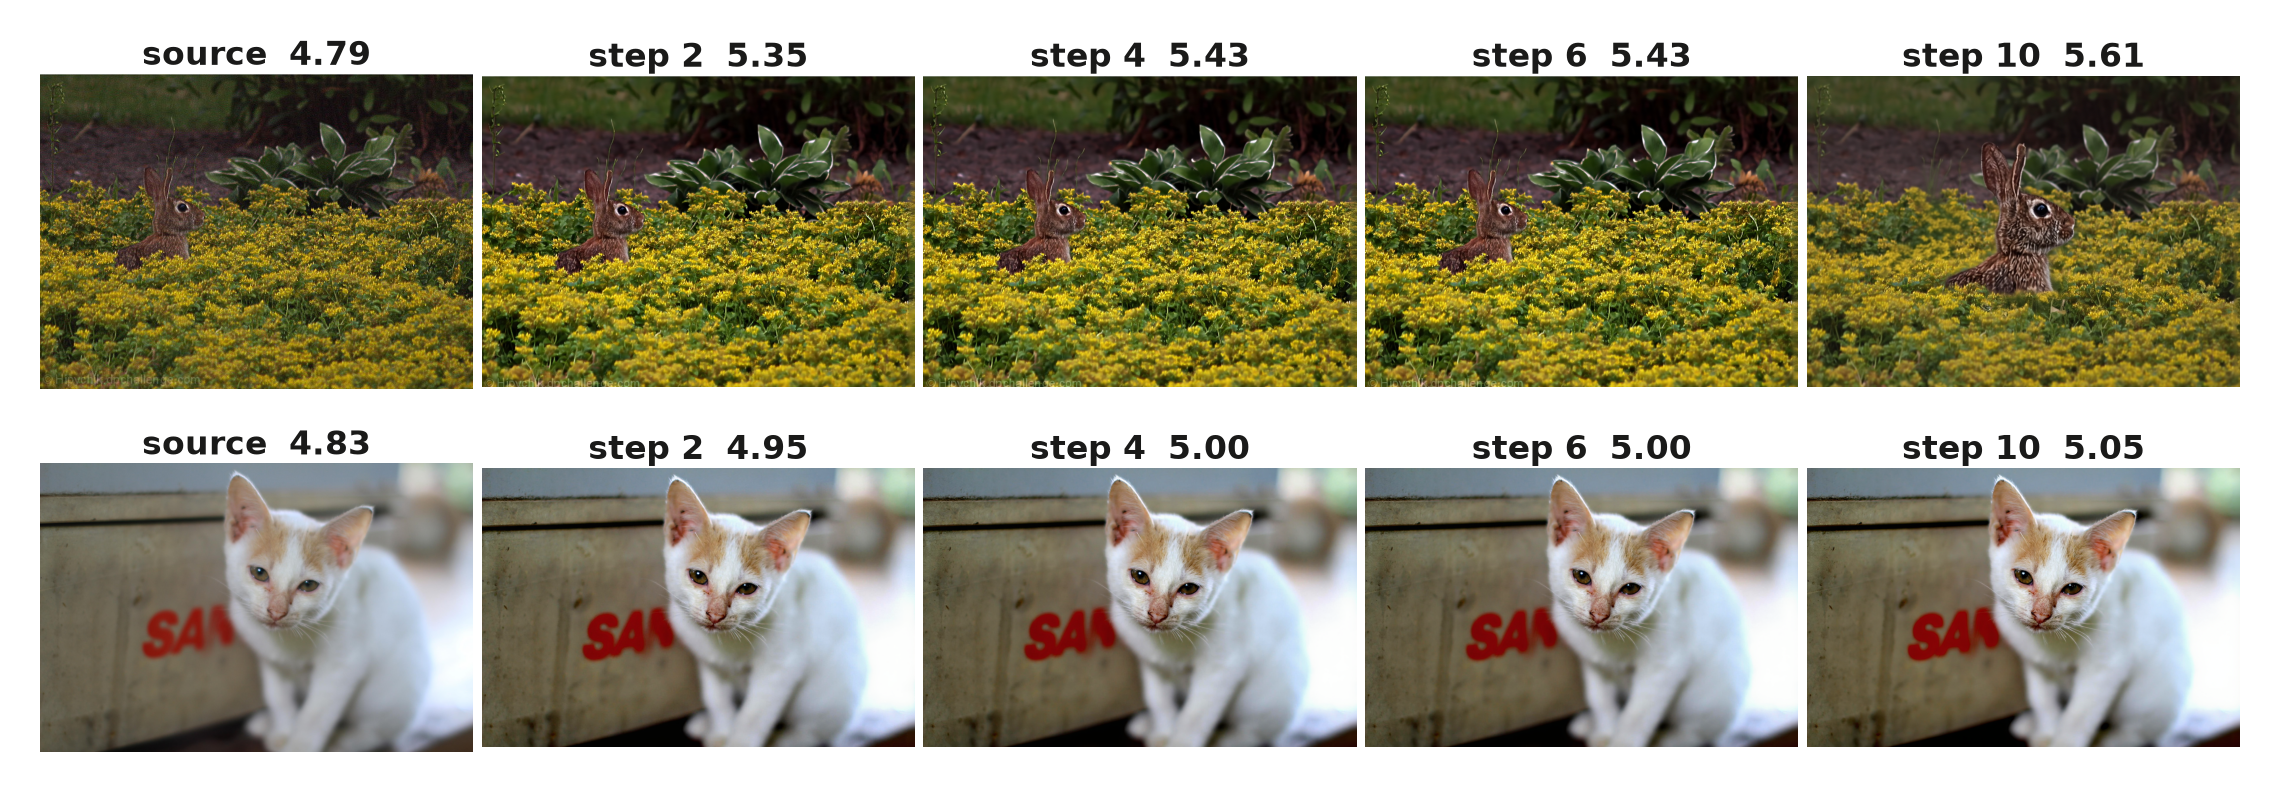
\includegraphics[width=\linewidth]{figs/pf_progression.png}
  \caption{\textbf{The loop over time.} The committed best-so-far image after refinement steps 0-10 for the \textsc{autopolish} critic, with the held-out aesthetic score above each cell. The audience's complaints accumulate across steps, so the edits arrive as visible increments rather than one jump, and the score rises monotonically by construction.}
  \label{fig:c4prog}
\end{figure}

\section{Conclusion}

This work is ultimately about \emph{agency}: who decides whether an image is good, and how much of that decision a creator hands over. Our premise is that there is no single verdict to hand over, because taste is plural. What we conclude is that this plurality can be simulated: a frozen model given personas, and listened to in numbers, is faithful to how a group would respond. And a reaction that can be simulated can be consulted while the work is still being made, which is what turns an audience into a critic. What that offers a creator is not a score but a voice they can hear and disagree with: the audience speaks, and the creator decides.

\newpage
\begin{ack}
Omitted for anonymous review.
\end{ack}


\begingroup
\small
\begin{thebibliography}{99}

\bibitem{argyle2023}
Argyle, L.P., Busby, E.C., Fulda, N., Gubler, J.R., Rytting, C.\ and Wingate, D.\ (2023)
Out of one, many: Using language models to simulate human samples.
{\it Political Analysis} {\bf 31}(3):337--351.

\bibitem{uma2021}
Uma, A.N., Fornaciari, T., Hovy, D., Paun, S., Plank, B.\ and Poesio, M.\ (2021)
Learning from disagreement: A survey.
{\it Journal of Artificial Intelligence Research} {\bf 72}:1385--1470.

\bibitem{plank2022}
Plank, B.\ (2022)
The ``problem'' of human label variation: On ground truth in data, modeling and evaluation.
In {\it Proceedings of the 2022 Conference on Empirical Methods in Natural Language Processing (EMNLP)}.

\bibitem{yang2022para}
Yang, Y., Xu, L., Li, L., Qie, N., Li, Y., Zhang, P.\ and Guo, Y.\ (2022)
Personalized image aesthetics assessment with rich attributes.
In {\it Proceedings of the IEEE/CVF Conference on Computer Vision and Pattern Recognition (CVPR)}.

\bibitem{murray2012ava}
Murray, N., Marchesotti, L.\ and Perronnin, F.\ (2012)
AVA: A large-scale database for aesthetic visual analysis.
In {\it Proceedings of the IEEE Conference on Computer Vision and Pattern Recognition (CVPR)}.

\bibitem{ke2023vila}
Ke, J., Ye, K., Yu, J., Wu, Y., Milanfar, P.\ and Yang, F.\ (2023)
VILA: Learning image aesthetics from user comments with vision-language pretraining.
In {\it Proceedings of the IEEE/CVF Conference on Computer Vision and Pattern Recognition (CVPR)}.

\bibitem{wu2024qalign}
Wu, H., Zhang, Z., Zhang, W., Chen, C., Liao, L., Li, C., Gao, Y., Wang, A., Zhang, E., Sun, W.,
Yan, Q., Min, X., Zhai, G.\ and Lin, W.\ (2024)
Q-Align: Teaching LMMs for visual scoring via discrete text-defined levels.
In {\it Proceedings of the 41st International Conference on Machine Learning (ICML)}.

\bibitem{rapidata2024}
Rapidata AG (2024)
700k human preference dataset: FLUX.1, Stable Diffusion 3, MidJourney and DALL$\cdot$E 3.
Hugging Face dataset.
\url{https://huggingface.co/datasets/Rapidata/700k_Human_Preference_Dataset_FLUX_SD3_MJ_DALLE3}

\bibitem{wang2024qwen2vl}
Wang, P., Bai, S., Tan, S., Wang, S., Fan, Z., Bai, J., Chen, K., Liu, X., Wang, J., Ge, W.,
Fan, Y., Dang, K., Du, M., Ren, X., Men, R., Liu, D., Zhou, C., Zhou, J.\ and Lin, J.\ (2024)
Qwen2-VL: Enhancing vision-language model's perception of the world at any resolution.
{\it arXiv preprint arXiv:2409.12191}.

\bibitem{flux2024}
Black Forest Labs, Batifol, S., Blattmann, A., Boesel, F., Consul, S., Diagne, C., Dockhorn, T.,
English, J., English, Z., Esser, P., Kulal, S., Lacey, K., Levi, Y., Li, C., Lorenz, D.,
M\"uller, J., Podell, D., Rombach, R., Saini, H., Sauer, A.\ and Smith, L.\ (2025)
FLUX.1 Kontext: Flow matching for in-context image generation and editing in latent space.
{\it arXiv preprint arXiv:2506.15742}.

\bibitem{schuhmann2022}
Schuhmann, C., Beaumont, R., Vencu, R., Gordon, C., Wightman, R., Cherti, M., Coombes, T.,
Katta, A., Mullis, C., Wortsman, M., Schramowski, P., Kundurthy, S., Crowson, K., Schmidt, L.,
Kaczmarczyk, R.\ and Jitsev, J.\ (2022)
LAION-5B: An open large-scale dataset for training next generation image-text models.
In {\it Advances in Neural Information Processing Systems 35 (NeurIPS), Datasets and Benchmarks Track}.

\bibitem{xu2023imagereward}
Xu, J., Liu, X., Wu, Y., Tong, Y., Li, Q., Ding, M., Tang, J.\ and Dong, Y.\ (2023)
ImageReward: Learning and evaluating human preferences for text-to-image generation.
In {\it Advances in Neural Information Processing Systems 36 (NeurIPS)}.

\bibitem{kirstain2023pickapic}
Kirstain, Y., Polyak, A., Singer, U., Matiana, S., Penna, J.\ and Levy, O.\ (2023)
Pick-a-Pic: An open dataset of user preferences for text-to-image generation.
In {\it Advances in Neural Information Processing Systems 36 (NeurIPS)}.

\bibitem{black2024ddpo}
Black, K., Janner, M., Du, Y., Kostrikov, I.\ and Levine, S.\ (2024)
Training diffusion models with reinforcement learning.
In {\it International Conference on Learning Representations (ICLR)}.

\bibitem{wallace2024dpo}
Wallace, B., Dang, M., Rafailov, R., Zhou, L., Lou, A., Purushwalkam, S., Ermon, S., Xiong, C.,
Joty, S.\ and Naik, N.\ (2024)
Diffusion model alignment using direct preference optimization.
In {\it Proceedings of the IEEE/CVF Conference on Computer Vision and Pattern Recognition (CVPR)}.

\bibitem{kong2016aadb}
Kong, S., Shen, X., Lin, Z., Mech, R.\ and Fowlkes, C.\ (2016)
Photo aesthetics ranking network with attributes and content adaptation.
In {\it Proceedings of the European Conference on Computer Vision (ECCV)}.

\bibitem{chang2017pccd}
Chang, K.-Y., Lu, K.-H.\ and Chen, C.-S.\ (2017)
Aesthetic critiques generation for photos.
In {\it Proceedings of the IEEE International Conference on Computer Vision (ICCV)}.

\bibitem{kang2020eva}
Kang, C., Valenzise, G.\ and Dufaux, F.\ (2020)
EVA: An explainable visual aesthetics dataset.
In {\it Proceedings of the Joint Workshop on Aesthetic and Technical Quality Assessment of
Multimedia and Media Analytics for Societal Trends (ATQAM/MAST), ACM International Conference
on Multimedia}, pp.\ 5--13.

\bibitem{maerten2025lapis}
Maerten, A.-S., Chen, L.-W., De Winter, S., Bossens, C.\ and Wagemans, J.\ (2025)
LAPIS: A novel dataset for personalized image aesthetic assessment.
In {\it Proceedings of the IEEE/CVF Conference on Computer Vision and Pattern Recognition (CVPR)
Workshops, Workshop on AI for Creative Visual Content Generation, Editing and Understanding (CVEU)}.

\bibitem{talebi2018nima}
Talebi, H.\ and Milanfar, P.\ (2018)
NIMA: Neural image assessment.
{\it IEEE Transactions on Image Processing} {\bf 27}(8):3998--4011.

\bibitem{jin2018cjs}
Jin, X., Wu, L., Li, X., Chen, S., Peng, S., Chi, J., Ge, S., Song, C.\ and Zhao, G.\ (2018)
Predicting aesthetic score distribution through cumulative Jensen-Shannon divergence.
In {\it Proceedings of the AAAI Conference on Artificial Intelligence (AAAI)}.

\bibitem{ren2017personalized}
Ren, J., Shen, X., Lin, Z., Mech, R.\ and Foran, D.J.\ (2017)
Personalized image aesthetics.
In {\it Proceedings of the IEEE International Conference on Computer Vision (ICCV)}.

\bibitem{zhu2022meta}
Zhu, H., Li, L., Wu, J., Zhao, S., Ding, G.\ and Shi, G.\ (2022)
Personalized image aesthetics assessment via meta-learning with bilevel gradient optimization.
{\it IEEE Transactions on Cybernetics} {\bf 52}(3):1798--1811.

\bibitem{wu2024qbench}
Wu, H., Zhang, Z., Zhang, E., Chen, C., Liao, L., Wang, A., Li, C., Sun, W., Yan, Q., Zhai, G.\
and Lin, W.\ (2024)
Q-Bench: A benchmark for general-purpose foundation models on low-level vision.
In {\it International Conference on Learning Representations (ICLR)}.

\bibitem{huang2024aesbench}
Huang, Y., Yuan, Q., Sheng, X., Yang, Z., Wu, H., Chen, P., Yang, Y., Li, L.\ and Lin, W.\ (2024)
AesBench: An expert benchmark for multimodal large language models on image aesthetics perception.
{\it arXiv preprint arXiv:2401.08276}.

\bibitem{zhou2024uniaa}
Zhou, Z., Wang, Q., Lin, B., Su, Y., Chen, R., Tao, X., Zheng, A., Yuan, L., Wan, P.\ and
Zhang, D.\ (2024)
UNIAA: A unified multi-modal image aesthetic assessment baseline and benchmark.
{\it arXiv preprint arXiv:2404.09619}.

\bibitem{huang2024aesexpert}
Huang, Y., Sheng, X., Yang, Z., Yuan, Q., Duan, Z., Chen, P., Li, L., Lin, W.\ and Shi, G.\ (2024)
AesExpert: Towards multi-modality foundation model for image aesthetics perception.
In {\it Proceedings of the 32nd ACM International Conference on Multimedia (ACM MM)}.

\bibitem{bisbee2024synthetic}
Bisbee, J., Clinton, J.D., Dorff, C., Kenkel, B.\ and Larson, J.M.\ (2024)
Synthetic replacements for human survey data? The perils of large language models.
{\it Political Analysis} {\bf 32}(4):401--416.

\bibitem{santurkar2023whose}
Santurkar, S., Durmus, E., Ladhak, F., Lee, C., Liang, P.\ and Hashimoto, T.\ (2023)
Whose opinions do language models reflect?
In {\it Proceedings of the 40th International Conference on Machine Learning (ICML)}.

\bibitem{cheng2023compost}
Cheng, M., Piccardi, T.\ and Yang, D.\ (2023)
CoMPosT: Characterizing and evaluating caricature in LLM simulations.
In {\it Proceedings of the 2023 Conference on Empirical Methods in Natural Language Processing (EMNLP)}.

\bibitem{fan2023dpok}
Fan, Y., Watkins, O., Du, Y., Liu, H., Ryu, M., Boutilier, C., Abbeel, P., Ghavamzadeh, M.,
Lee, K.\ and Lee, K.\ (2023)
DPOK: Reinforcement learning for fine-tuning text-to-image diffusion models.
In {\it Advances in Neural Information Processing Systems 36 (NeurIPS)}.

\bibitem{clark2024draft}
Clark, K., Vicol, P., Swersky, K.\ and Fleet, D.J.\ (2024)
Directly fine-tuning diffusion models on differentiable rewards.
In {\it International Conference on Learning Representations (ICLR)}.

\bibitem{prabhudesai2023alignprop}
Prabhudesai, M., Goyal, A., Pathak, D.\ and Fragkiadaki, K.\ (2023)
Aligning text-to-image diffusion models with reward backpropagation.
{\it arXiv preprint arXiv:2310.03739}.

\bibitem{madaan2023selfrefine}
Madaan, A., Tandon, N., Gupta, P., Hallinan, S., Gao, L., Wiegreffe, S., Alon, U., Dziri, N.,
Prabhumoye, S., Yang, Y., Gupta, S., Majumder, B.P., Hermann, K., Welleck, S., Yazdanbakhsh, A.\
and Clark, P.\ (2023)
Self-Refine: Iterative refinement with self-feedback.
In {\it Advances in Neural Information Processing Systems 36 (NeurIPS)}.

\bibitem{shinn2023reflexion}
Shinn, N., Cassano, F., Berman, E., Gopinath, A., Narasimhan, K.\ and Yao, S.\ (2023)
Reflexion: Language agents with verbal reinforcement learning.
In {\it Advances in Neural Information Processing Systems 36 (NeurIPS)}.

\bibitem{gou2024critic}
Gou, Z., Shao, Z., Gong, Y., Shen, Y., Yang, Y., Duan, N.\ and Chen, W.\ (2024)
CRITIC: Large language models can self-correct with tool-interactive critiquing.
In {\it International Conference on Learning Representations (ICLR)}.

\bibitem{wu2024sld}
Wu, T.-H., Lian, L., Gonzalez, J.E., Li, B.\ and Darrell, T.\ (2024)
Self-correcting LLM-controlled diffusion models.
In {\it Proceedings of the IEEE/CVF Conference on Computer Vision and Pattern Recognition (CVPR)}.

\bibitem{wang2024genartist}
Wang, Z., Li, A., Li, Z.\ and Liu, X.\ (2024)
GenArtist: Multimodal LLM as an agent for unified image generation and editing.
In {\it Advances in Neural Information Processing Systems 37 (NeurIPS)}.

\bibitem{brooks2023instructpix2pix}
Brooks, T., Holynski, A.\ and Efros, A.A.\ (2023)
InstructPix2Pix: Learning to follow image editing instructions.
In {\it Proceedings of the IEEE/CVF Conference on Computer Vision and Pattern Recognition (CVPR)}.

\bibitem{xu2024selfbias}
Xu, W., Zhu, G., Zhao, X., Pan, L., Li, L.\ and Wang, W.Y.\ (2024)
Pride and prejudice: LLM amplifies self-bias in self-refinement.
In {\it Proceedings of the 62nd Annual Meeting of the Association for Computational Linguistics
(ACL), Volume 1: Long Papers}, pp.\ 15474--15492.

\bibitem{radford2021}
Radford, A., Kim, J.W., Hallacy, C., Ramesh, A., Goh, G., Agarwal, S., Sastry, G., Askell, A.,
Mishkin, P., Clark, J., Krueger, G.\ and Sutskever, I.\ (2021)
Learning transferable visual models from natural language supervision.
In {\it Proceedings of the 38th International Conference on Machine Learning (ICML)}.

\bibitem{oquab2023}
Oquab, M., Darcet, T., Moutakanni, T., Vo, H., Szafraniec, M., Khalidov, V., Fernandez, P.,
Haziza, D., Massa, F., El-Nouby, A., Assran, M., Ballas, N., Galuba, W., Howes, R., Huang, P.-Y.,
Li, S.-W., Misra, I., Rabbat, M., Sharma, V., Synnaeve, G., Xu, H., J\'egou, H., Mairal, J.,
Labatut, P., Joulin, A.\ and Bojanowski, P.\ (2024)
DINOv2: Learning robust visual features without supervision.
{\it Transactions on Machine Learning Research}.

\bibitem{niculescu2005}
Niculescu-Mizil, A.\ and Caruana, R.\ (2005)
Predicting good probabilities with supervised learning.
In {\it Proceedings of the 22nd International Conference on Machine Learning (ICML)}.

\bibitem{shrout1979}
Shrout, P.E.\ and Fleiss, J.L.\ (1979)
Intraclass correlations: Uses in assessing rater reliability.
{\it Psychological Bulletin} {\bf 86}(2):420--428.

\bibitem{pamela2026}
Maerten, A.-S., Verwiebe, J., Karthik, S., Prabhu, A., Wagemans, J.\ and Bethge, M.\ (2026)
Personalizing text-to-image generation to individual taste.
{\it arXiv preprint arXiv:2604.07427}.

\bibitem{aesbiasbench2025}
Li, K., Po, L.-M., Yang, H., Xu, X., Liu, K.\ and Zhao, Y.\ (2025)
AesBiasBench: Evaluating bias and alignment in multimodal language models for personalized
image aesthetic assessment.
In {\it Proceedings of the 2025 Conference on Empirical Methods in Natural Language
Processing (EMNLP)}.

\bibitem{hu2022lora}
Hu, E.J., Shen, Y., Wallis, P., Allen-Zhu, Z., Li, Y., Wang, S., Wang, L.\ and Chen, W.\ (2022)
LoRA: Low-rank adaptation of large language models.
In {\it International Conference on Learning Representations (ICLR)}.

\bibitem{salganik2006}
Salganik, M.J., Dodds, P.S.\ and Watts, D.J.\ (2006)
Experimental study of inequality and unpredictability in an artificial cultural market.
{\it Science} {\bf 311}(5762):854--856.

\end{thebibliography}
\endgroup


%%%%%%%%%%%%%%%%%%%%%%%%%%%%%%%%%%%%%%%%%%%%%%%%%%%%%%%%%%%%
% ------------------------ Supplementary Material ------------------------
%%%%%%%%%%%%%%%%%%%%%%%%%%%%%%%%%%%%%%%%%%%%%%%%%%%%%%%%%%%%
\newpage
\begin{center}
  \rule{\textwidth}{4pt}\\[0.16in]
  {\bfseries\fontsize{14}{17}\selectfont Supplementary Material\\[5pt]}
  {\bfseries\fontsize{17}{21}\selectfont AutoPolish: Improving Visual Aesthetics\\ with Synthetic Audience Critique\\[0.14in]}
  \rule{\textwidth}{1pt}
\end{center}
\vspace{1.1em}

\appendix
\setcounter{section}{0}
\renewcommand{\thesection}{S\arabic{section}}
\setcounter{figure}{0}
\renewcommand{\thefigure}{S\arabic{figure}}
\setcounter{table}{0}
\renewcommand{\thetable}{S\arabic{table}}

This supplement gives the dataset details, the per-experiment figures behind the composite panels of the main paper, additional analyses and ablations, the limitations and honest negatives in full (Section~\ref{sec:limits}) with the future directions they point to (Section~\ref{sup:future}), and finally the exact prompts with two worked examples of the AutoPolish loop. All figures share the palette used in the main text, and every number carries the same 1000-sample bootstrap, clustered by rater and image.

\section{Background and related work in full}
\label{sup:related}

\subsection{Aesthetics as a multidimensional and subjective signal}
Computational work on image aesthetics is usually framed as predicting a single quality score, yet the field's own foundational resources show that the target is neither one-dimensional nor universal. AVA \citep{murray2012ava} supplies roughly 250k photographs with score histograms over about 200 voters each, together with semantic and photographic-style labels. AADB \citep{kong2016aadb} adds eleven interpretable attributes, among them interesting content, object emphasis, lighting, color harmony, depth of field, motion blur, rule of thirds, balancing element, repetition, symmetry, and vivid color, and it retains per-rater identifiers so that individual rankings can be studied rather than averaged away. PCCD \citep{chang2017pccd} pairs images with professional critiques along seven axes, and EVA \citep{kang2020eva} collects about 137k votes with four attribute dimensions plus difficulty judgments. The recurring finding across these resources is that a mean opinion score compresses a rich, disagreement-laden distribution into one number.

Two lines of work take that compression seriously. Distribution-based methods predict the full histogram instead of its mean: NIMA \citep{talebi2018nima} optimizes an earth-mover distance loss over the rating distribution, and CJS-CNN \citep{jin2018cjs} reweights by rater reliability. Personalized methods instead model who is rating. Ren et al.\ \citep{ren2017personalized} decompose a score into a generic component and a learned per-user offset, Zhu et al.\ \citep{zhu2022meta} use meta-learning for few-shot adaptation to a new user, and PARA \citep{yang2022para} provides 31k images and 438k per-user annotations with explicit subject traits such as age, gender, education, artistic and photographic experience, and Big-Five personality. This literature establishes that individual taste is partly predictable from viewer attributes, but it stops at the individual: it does not ask what a \emph{population} of viewers would say, nor does it use the predicted reaction to change an image.

\subsection{Vision-language models as aesthetic judges}
CLIP-based scorers made zero-shot aesthetic prediction practical, and the LAION aesthetic predictor \citep{schuhmann2022} became the de facto filter for web-scale image corpora and a common reward for generative fine-tuning. VILA \citep{ke2023vila} pretrains on image-comment pairs and adapts with a lightweight residual adapter for both score and comment generation. Instruction-tuned multimodal LLMs then made scoring conversational: Q-Bench \citep{wu2024qbench} and Q-Align \citep{wu2024qalign} show that mapping continuous quality onto discrete text-defined levels, from ``excellent'' to ``bad'', yields state-of-the-art mean-opinion-score prediction and transfers across image quality assessment, image aesthetics assessment, and video. AesBench \citep{huang2024aesbench}, UNIAA \citep{zhou2024uniaa}, and AesExpert \citep{huang2024aesexpert} benchmark and instruction-tune specifically for aesthetic perception, consistently reporting that general-purpose multimodal LLMs still trail humans on fine-grained aesthetic reasoning. All of this work targets a single consensus judgment; none simulates a distribution of viewers.

\subsection{Simulating human populations with language models}
In the text-only setting, language models have been used as stand-ins for human respondents. Argyle et al.\ \citep{argyle2023} show that conditioning GPT-3 on demographic backstories reproduces ANES response distributions with high fidelity, a property they call algorithmic fidelity. Subsequent work is more skeptical. Bisbee et al.\ \citep{bisbee2024synthetic} find that synthetic ANES responses have systematically lower variance than human data and are sensitive to prompt phrasing and model version. Santurkar et al.\ \citep{santurkar2023whose} introduce OpinionQA and show that language-model opinion distributions are badly misaligned with several US demographic groups, with persona steering only partially correcting it. Cheng et al.\ \citep{cheng2023compost} further show that persona prompts can amplify caricature. Two consequences matter for us. First, aggregate-level simulation is more trustworthy than individual-level simulation. Second, calibration and explicit variance controls are prerequisites, not refinements. This literature is almost entirely text; whether persona conditioning transfers to \emph{visual} aesthetic judgment is open.

\subsection{Feedback loops for image generation and editing}
Reward-driven refinement of generative models is now standard. ImageReward \citep{xu2023imagereward} trains a preference model on 137k comparisons and fine-tunes diffusion through reward feedback learning; DPOK \citep{fan2023dpok} and DDPO \citep{black2024ddpo} apply policy-gradient reinforcement learning against a reward; DRaFT \citep{clark2024draft} and AlignProp \citep{prabhudesai2023alignprop} backpropagate differentiable rewards; and Diffusion-DPO \citep{wallace2024dpo} removes the explicit reward model through direct preference optimization on Pick-a-Pic \citep{kirstain2023pickapic}. In parallel, self-refinement with language feedback, including Self-Refine \citep{madaan2023selfrefine}, Reflexion \citep{shinn2023reflexion}, and CRITIC \citep{gou2024critic}, established the iterative critique-and-revise pattern, and multimodal variants such as SLD \citep{wu2024sld} and GenArtist \citep{wang2024genartist} use a vision-language model to detect faults and dispatch corrections. Instruction-based editors including InstructPix2Pix \citep{brooks2023instructpix2pix} and FLUX.1-Kontext \citep{flux2024} provide the actuator such loops require. Two gaps persist. First, every reward here is a scalar consensus signal, so none represents an audience. Second, when the same model both proposes and evaluates an edit, improvement can be self-fulfilling, a circularity that work on self-bias in language-model evaluation documents directly \citep{xu2024selfbias}.

\subsection{Positioning}
Our contribution sits at the intersection of these four lines. From personalized aesthetics we take viewer attributes seriously, but relocate the prediction target from the individual to the group. From population simulation with language models we take persona conditioning and the discipline of calibration, but move it from text surveys to visual aesthetic judgment. From the reward-optimization literature we take the loop, but replace the scalar consensus reward with a plural audience whose critique is natural language, and enforce a strict separation between the critic that proposes and the frozen, held-out judge that scores.


\section{Datasets}
Table~\ref{tab:data} gives the four corpora in full. The ordering that matters is persona richness, which decreases from PARA and LAPIS to EVA and which turns out to be the single best predictor of where persona-dependent claims hold.

\begin{table}[h]
  \caption{Datasets. Persona richness decreases from PARA/LAPIS to EVA, which proves to be the single best predictor of where the method works.}
  \label{tab:data}
  \centering
  \small
  \setlength{\tabcolsep}{5pt}
  \begin{tabular}{lllp{4.6cm}}
    \toprule
    Dataset & Content & Scale used & Persona fields \\
    \midrule
    PARA     & photographs        & 4{,}000 imgs / $\sim$52k ratings & age, gender, education, art \& photo exp., Big-Five \\
    EVA      & photographs (AVA)  & 4{,}070 imgs / 137k ratings      & age, gender, region, photographic level \\
    LAPIS    & paintings          & 4{,}000 imgs / 90k ratings       & nationality, art interest, age \\
    Rapidata & generated pairs    & 23k votes / 898 pairs / 120 ctry & per-vote country + language \\
    \bottomrule
  \end{tabular}
\end{table}

\section{The reliability ceiling}
Table~\ref{tab:ceiling} gives the per-dataset variance decomposition behind the main paper's ceiling argument: the reliability of a single rating, the reliability of the group mean, and the share of individual taste that persona attributes can explain at all.

\begin{table}[h]
  \caption{The ceiling. A single rating shares only a fraction of its variance with other raters, the group mean is highly reliable, and persona attributes explain only 1-4\% of individual taste, so the individual is near-noise and the group is the right target.}
  \label{tab:ceiling}
  \centering
  \small
  \begin{tabular}{lcccc}
    \toprule
    Dataset & ICC(1), one rating & ICC(k), group mean & between-image var. & persona-$\Delta R^2$ \\
    \midrule
    PARA  & 0.470 & \textbf{0.958} & 0.470 & 2.0\% \\
    EVA   & 0.223 & \textbf{0.906} & 0.223 & 0.9\% \\
    LAPIS & 0.188 & \textbf{0.839} & 0.188 & 4.0\% \\
    \bottomrule
  \end{tabular}
\end{table}

\section{Calibration in full: individual, group, and prior}
Figure~\ref{fig:cal} expands panel (a) of the main paper's audience figure to show the individual as well as the group. Out-of-fold isotonic calibration roughly halves group error and pushes the calibrated group (blue, fourth bar) below the population-mean prior (orange) on all three datasets, while the individual prediction, even after calibration, stays near-noise exactly as the ceiling analysis predicts.

\begin{figure}[h]
  \centering
  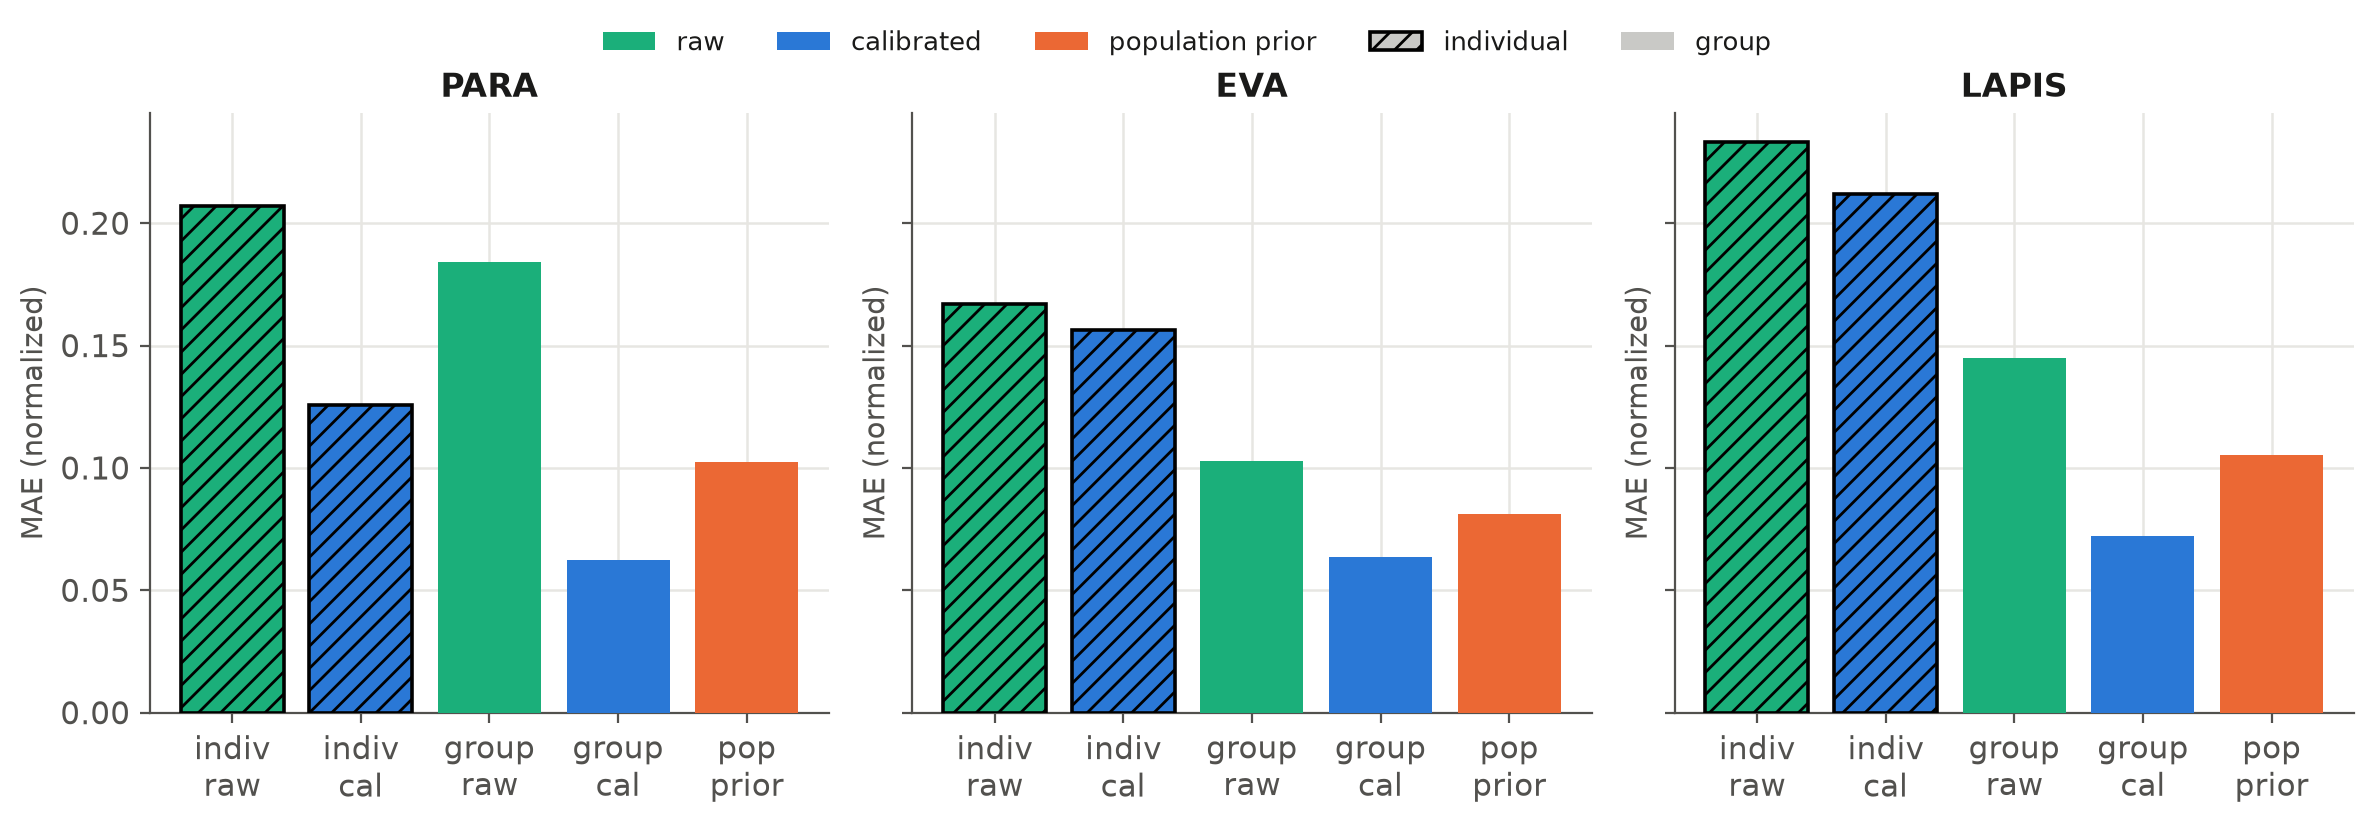
\includegraphics[width=0.98\linewidth]{figs/b4_calibration.png}
  \caption{\textbf{Calibration is what makes the aggregate beat the prior.} Normalized MAE for individual (hatched) and group (solid) predictions, raw versus calibrated, with the population-mean prior for reference. The calibrated group beats the prior on all three datasets; the individual does not, and cannot.}
  \label{fig:cal}
\end{figure}

\section{Calibration transfers across datasets}
The isotonic calibrator is fit out-of-fold on one dataset and evaluated on another (Figure~\ref{fig:xcal}). Every off-diagonal transfer sits far below the corresponding raw (uncalibrated) error, so a calibrator fit once on real images can be reused unchanged, which is exactly what licenses the ``fit once, reuse on generated images'' step behind the generated-image results.

\begin{figure}[h]
  \centering
  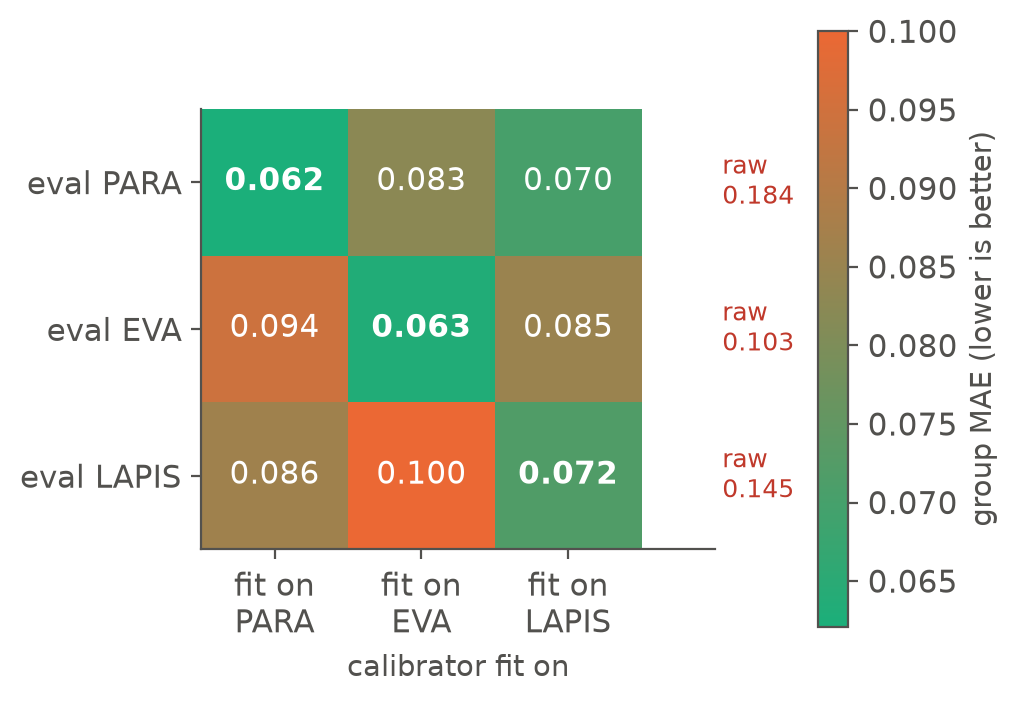
\includegraphics[width=0.66\linewidth]{figs/ax_calib_transfer.png}
  \caption{\textbf{Calibration transfers.} Calibrated group MAE when the isotonic map is fit on one dataset (columns) and evaluated on another (rows); the diagonal is the matched case. Every entry is far below the raw, uncalibrated error (red, right), so the correction is a general scale fix rather than a dataset-specific one.}
  \label{fig:xcal}
\end{figure}

\section{Why calibration is needed: the judge's central-tendency bias}
The raw judge concentrates its answers on a single value far more than humans do and, on the wider-scale datasets, uses less of the range (Figure~\ref{fig:style}). This response-style bias, not random error, is what inflates raw distributional error and is what out-of-fold calibration removes.

\begin{figure}[h]
  \centering
  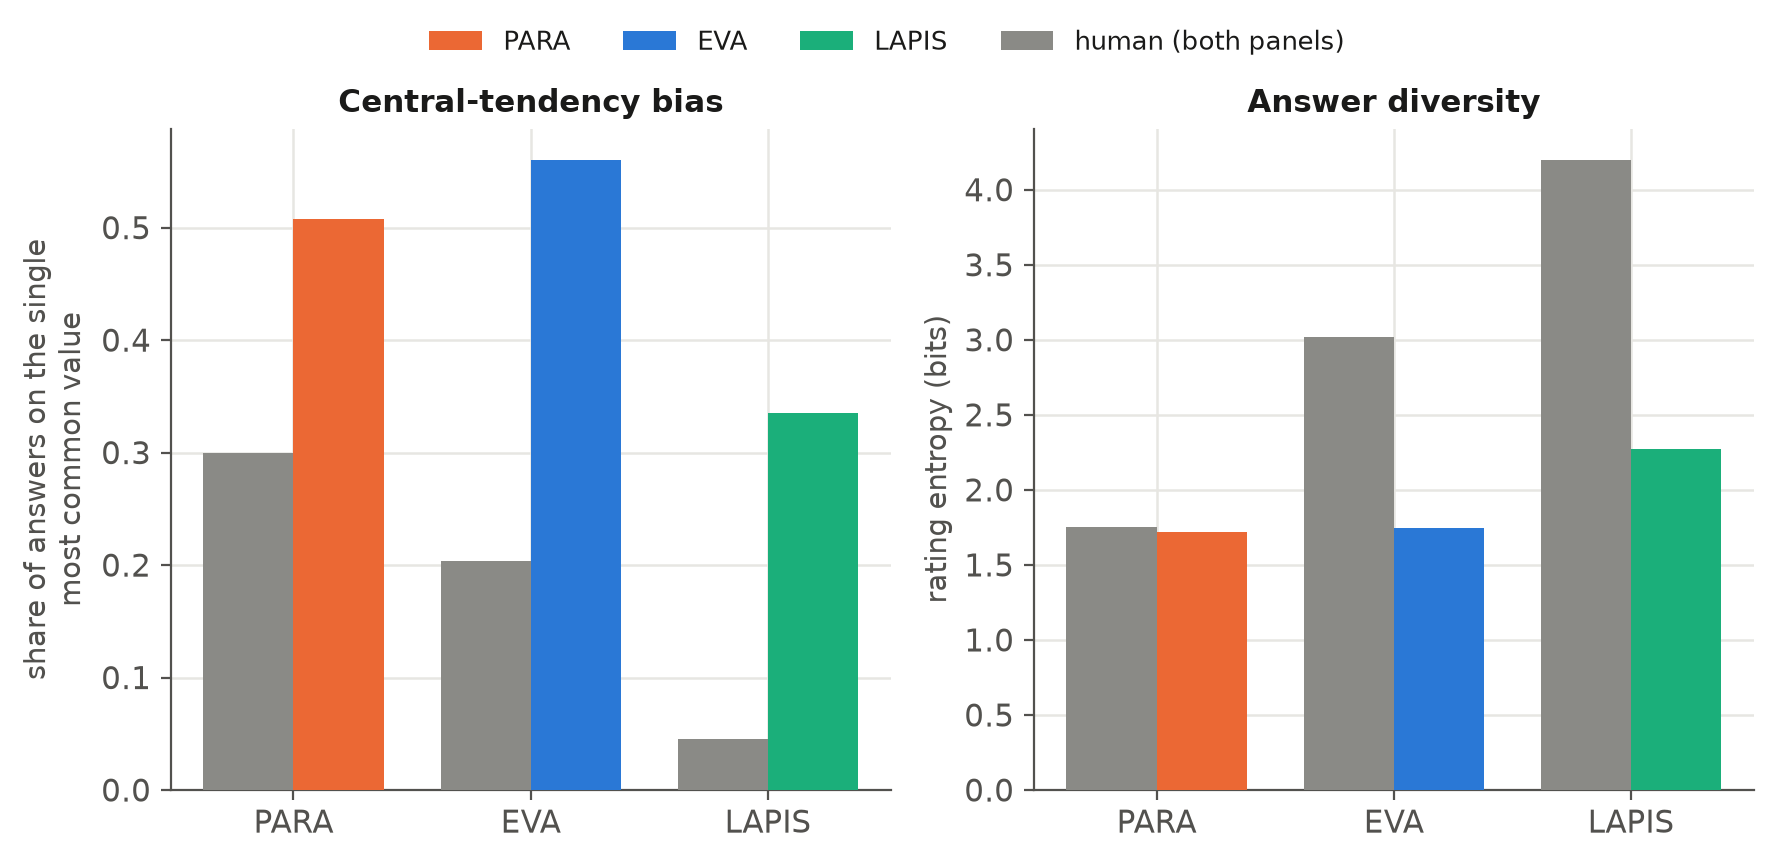
\includegraphics[width=0.86\linewidth]{figs/ax_response_style.png}
  \caption{\textbf{The judge has a central-tendency bias.} Left: the frozen VLM places a much larger share of its answers on the single most common rating than humans do. Right: its rating entropy is lower on the wider-scale datasets (EVA, LAPIS). Calibration corrects this scale and central-tendency mismatch.}
  \label{fig:style}
\end{figure}

\section{The persona moves the score}
Figure~\ref{fig:steer} shows the score-level steerability behind the claim that the persona is functional: persona-induced deviation plotted against the empirical group deviation, per dataset, with marker size proportional to slice support.

\begin{figure}[h]
  \centering
  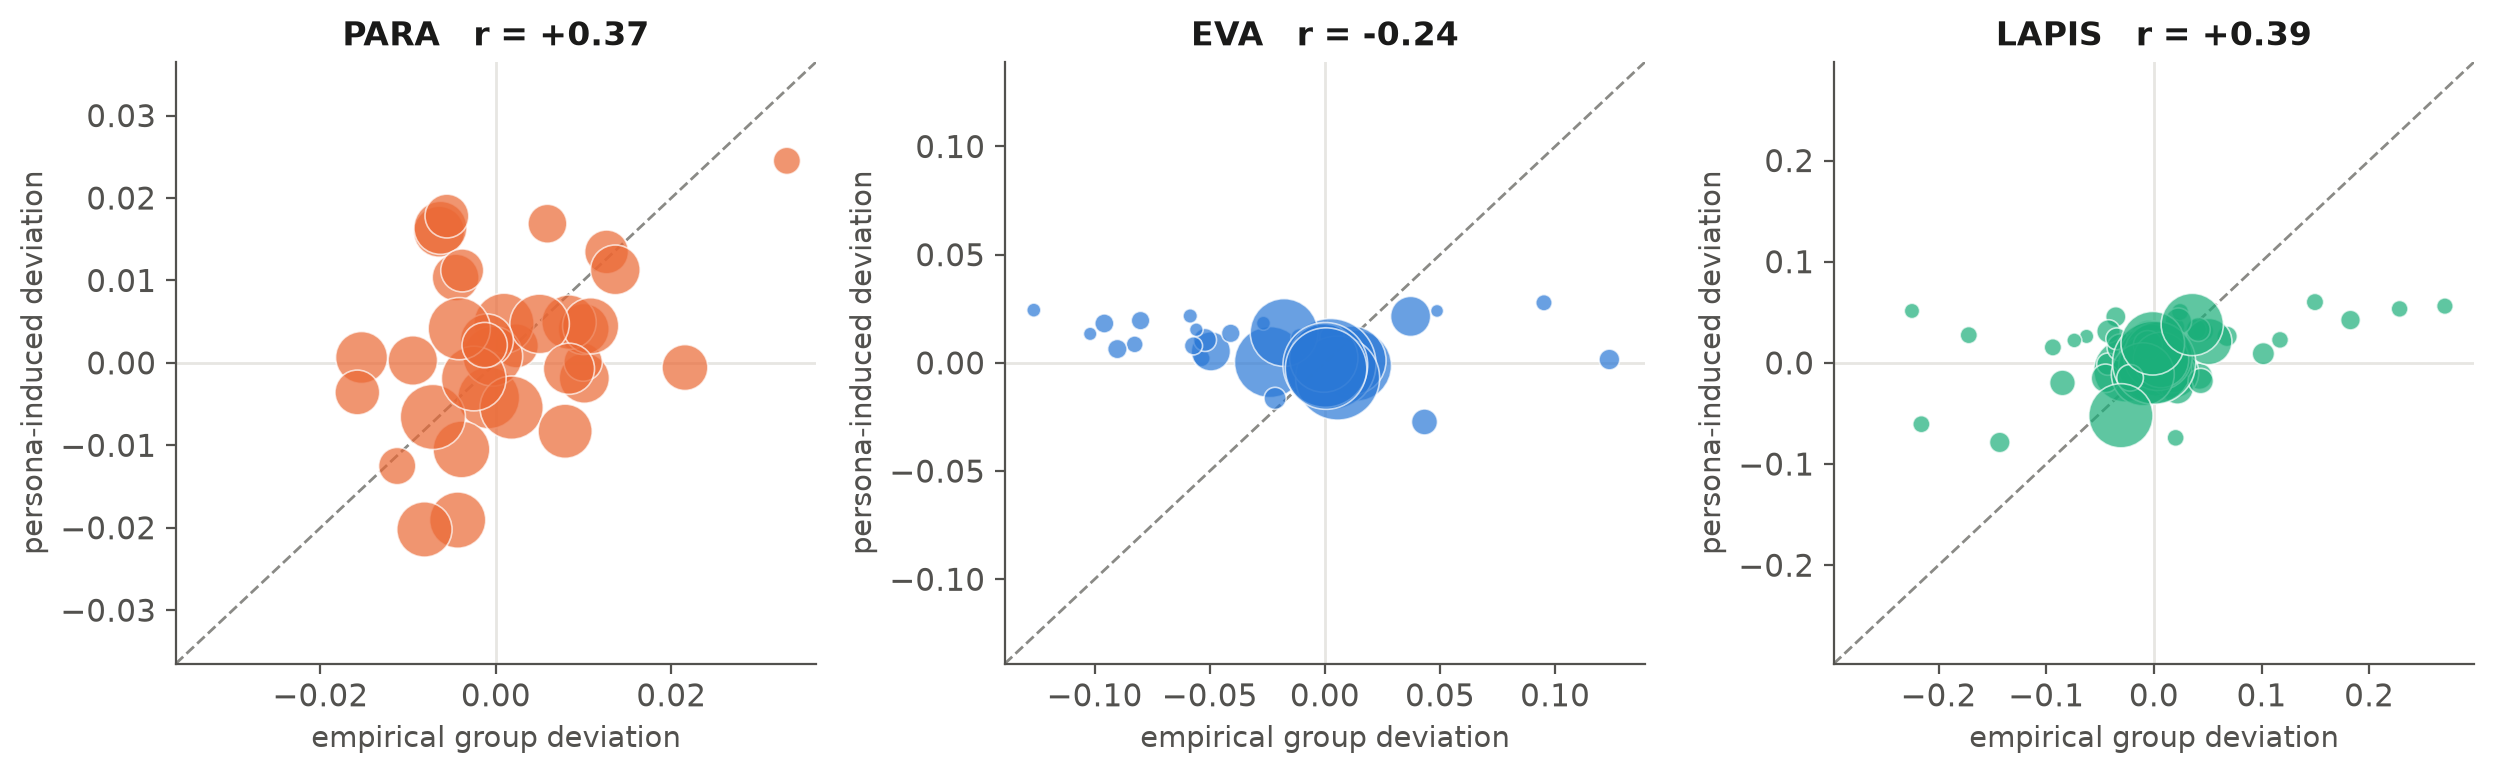
\includegraphics[width=0.95\linewidth]{figs/b1_steerability.png}
  \caption{\textbf{The persona is functional.} Persona-induced deviation against the empirical group deviation, per dataset; marker size is slice support. On the attribute-rich datasets the persona moves the judge in the direction the data says it should ($r{=}0.37$ on PARA, $0.39$ on LAPIS); on the thin-persona EVA it does not, matching the richness ordering.}
  \label{fig:steer}
\end{figure}

\section{The persona also steers the rationale language}
Beyond the numeric score, the persona reshapes the judge's free-text rationale (Figure~\ref{fig:rat}). A held-out probe recovers the rater's attribute from the generated rationale text well above chance for the persona judge on all three datasets, while the persona-blind control sits at chance, and the persona produces several times more distinct rationales. This is direct evidence that the persona is functional even where a coarse integer score hides it, as on EVA.

\begin{figure}[h]
  \centering
  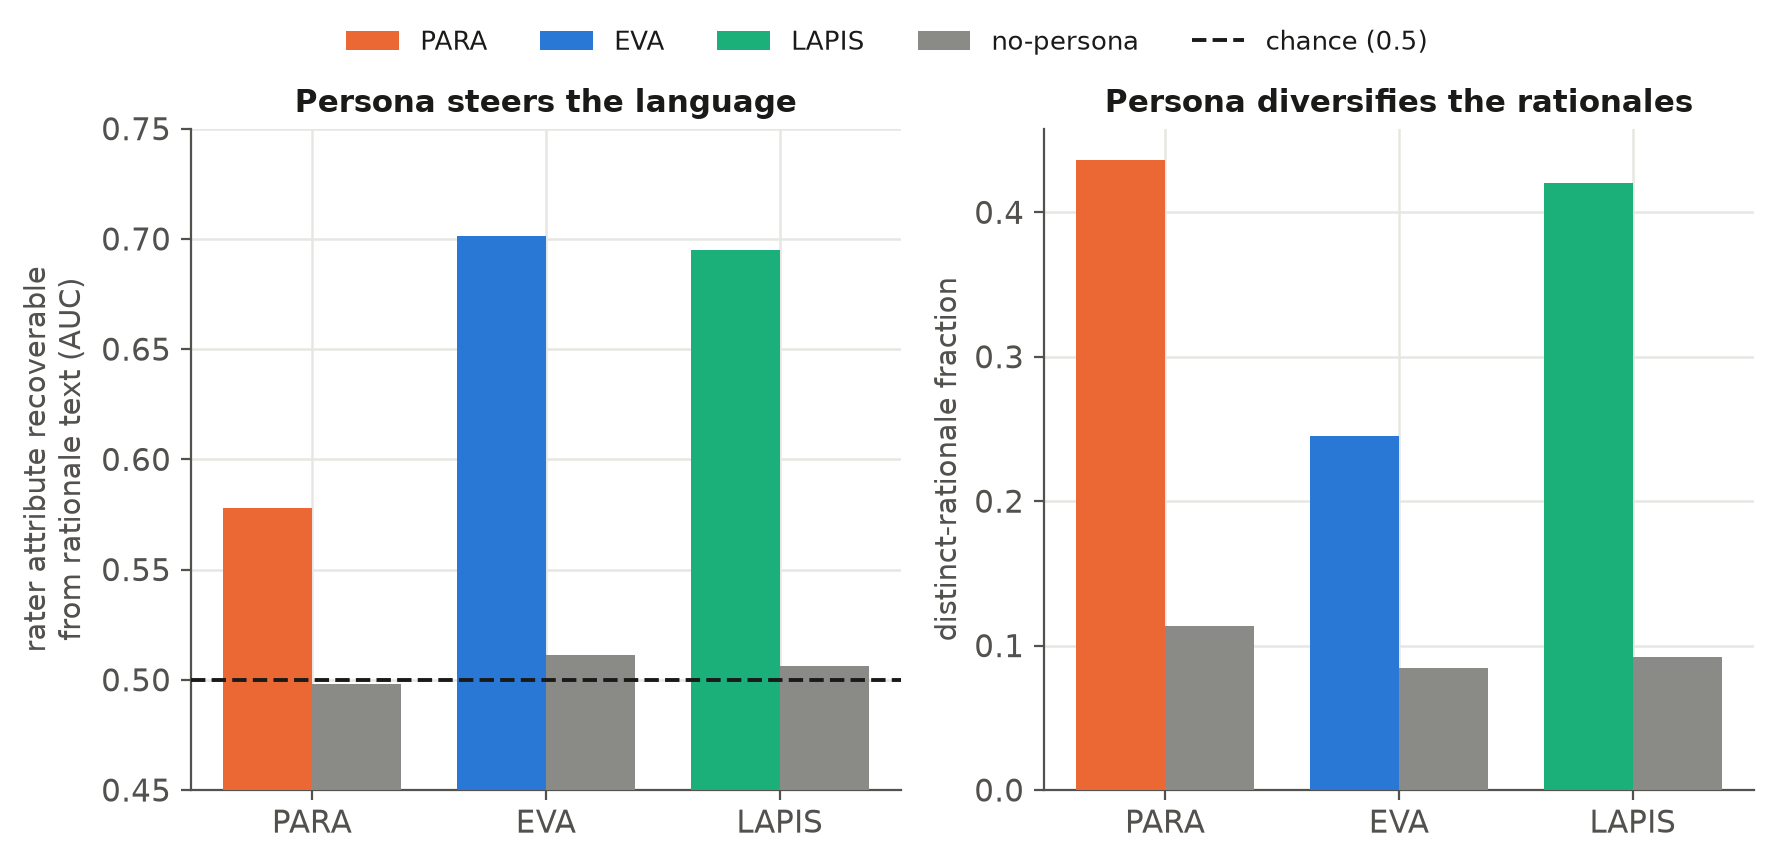
\includegraphics[width=0.86\linewidth]{figs/ax_rationale.png}
  \caption{\textbf{The persona is functional in the text.} Left: a probe recovers a rater's attribute from the generated rationale far above chance for the persona judge, but not for the persona-blind control. Right: the persona produces several times more distinct rationales. The persona is being computed even when the discrete score cannot express it.}
  \label{fig:rat}
\end{figure}

\section{The group beats the population prior on every rated axis}
Across all sixteen rated dimensions of the three datasets, the calibrated panel's group error is below the population-mean prior (Figure~\ref{fig:breadth}); a non-VLM collaborative-filtering baseline confirms from the other side that personalization buys little (warm-start gain of only $0.013$-$0.031$ MAE). Together these show the group signal is broad and real, not specific to the headline aesthetic axis.

\begin{figure}[h]
  \centering
  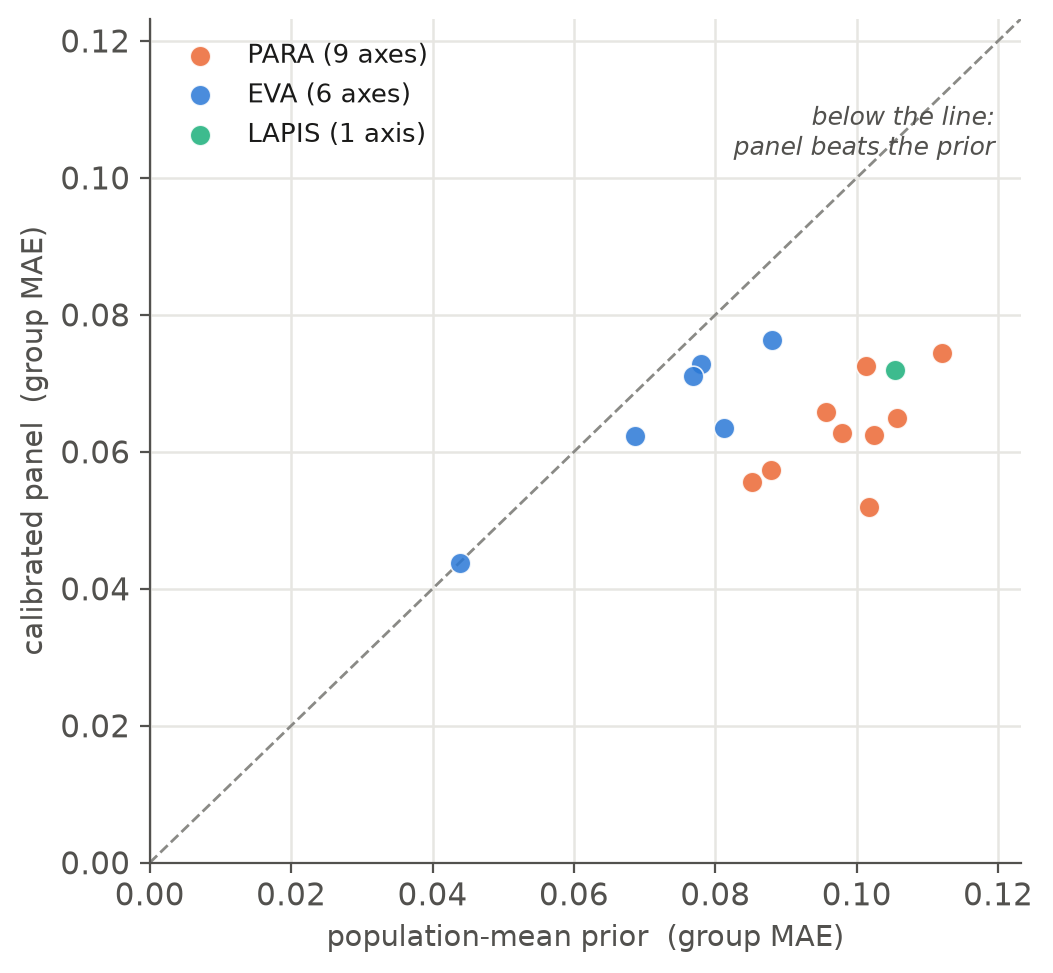
\includegraphics[width=0.56\linewidth]{figs/ax_breadth.png}
  \caption{\textbf{The group beats the prior everywhere.} Calibrated panel group MAE against the population-mean prior for all 16 rated axes across the three datasets. Every point but one lies below the diagonal, i.e.\ the panel is at least as accurate as the prior on essentially every dimension.}
  \label{fig:breadth}
\end{figure}

\section{Panel preference tracks the crowd on generated images}
Beyond the panel-size curve reported in the main text, the aggregated panel's per-pair preference correlates with the human crowd's win-rate at $r{=}+0.47$ (Figure~\ref{fig:c3scatter}). The aggregate is a real preference signal on generated content, even though between-country differences, a separate claim, do not transfer.

\begin{figure}[h]
  \centering
  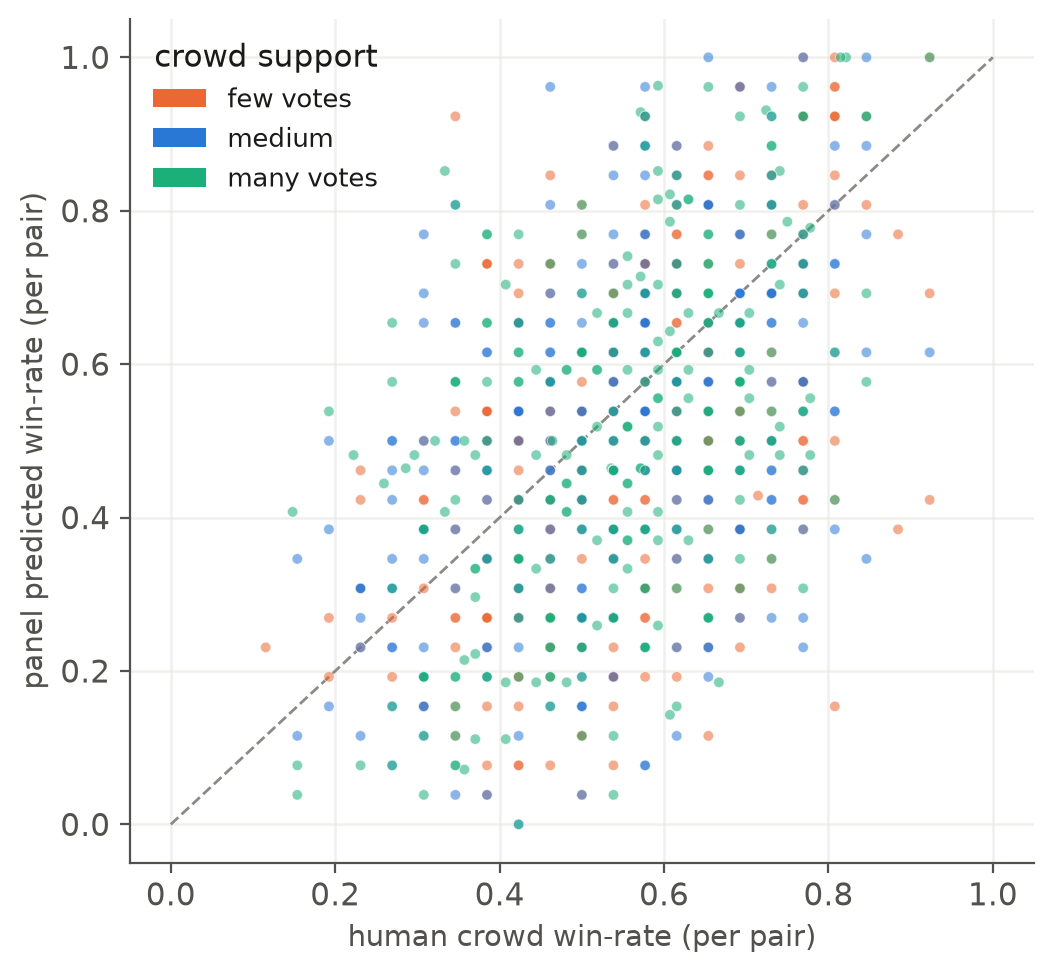
\includegraphics[width=0.52\linewidth]{figs/c3_aggregate_scatter.png}
  \caption{\textbf{Aggregated panel preference tracks the crowd.} Predicted panel preference against observed human win-rate over 898 AI-generated image pairs, points colored by crowd-support tercile; $r{=}+0.466$ (95\% CI $[0.415, 0.515]$).}
  \label{fig:c3scatter}
\end{figure}

\section{The headline is not a decoding artifact: temperature study}
Re-running at temperature $0.7$ leaves the between-group separation and the steerability essentially unchanged, while the panel-size curve stays flat under both settings (Table~\ref{tab:temp}). The flat panel-size curve on real images is therefore a decoding-collapse property of the backbone (roughly half of images give a point-mass panel), not evidence against aggregation, and the headline separation result is stable across decoding.

\begin{table}[h]
  \caption{Temperature robustness. Greedy (t$=$0) versus sampled (t$=$0.7) decoding. The separation and steerability barely move and the N-curve stays flat under both, so the headline is not a decoding artifact; the large degenerate-panel fraction on PARA/EVA explains the flat N-curve.}
  \label{tab:temp}
  \centering
  \small
  \setlength{\tabcolsep}{3.5pt}
  \begin{tabular}{llcccc}
    \toprule
    Dataset & decoding & degenerate panels & N-curve drop ($N{=}1{\to}20$) & separation (95\% CI) & steerability \\
    \midrule
    PARA  & t$=$0    & 0.48 & 0.003 & $+0.044\ [0.025, 0.064]$ & $+0.37$ \\
    PARA  & t$=$0.7  & 0.42 & 0.004 & $+0.040\ [0.027, 0.055]$ & $+0.39$ \\
    EVA   & t$=$0    & 0.51 & 0.003 & $-0.085\ [-0.103, -0.066]$ & $-0.24$ \\
    EVA   & t$=$0.7  & 0.53 & 0.003 & $-0.080\ [-0.099, -0.061]$ & $-0.27$ \\
    LAPIS & t$=$0    & 0.04 & 0.011 & $+0.166\ [0.149, 0.181]$ & $+0.39$ \\
    LAPIS & t$=$0.7  & 0.03 & 0.006 & $+0.172\ [0.156, 0.189]$ & $+0.41$ \\
    \bottomrule
  \end{tabular}
\end{table}

\section{Multiple-comparison correction}
The per-slice separations survive Holm correction across the full sweep of eight slice tests (Table~\ref{tab:holm}): six of eight are significant at $\alpha=0.05$, including every LAPIS slice and both PARA experience slices, while the two null slices (PARA age, EVA photographic level) fail as expected.

\begin{table}[h]
  \caption{Holm-corrected slice tests ($n=8$, $\alpha=0.05$). Six of eight between-group separations survive correction, including the nationality slice that the cross-cultural analysis builds on.}
  \label{tab:holm}
  \centering
  \small
  \begin{tabular}{llccc}
    \toprule
    Dataset & slice & separation $r$ & Holm-adjusted $p$ & survives \\
    \midrule
    LAPIS & age                   & $+0.102$ & $<10^{-3}$ & \checkmark \\
    LAPIS & art interest          & $+0.088$ & $<10^{-3}$ & \checkmark \\
    EVA   & age                   & $-0.079$ & $<10^{-3}$ & \checkmark \\
    LAPIS & nationality           & $+0.068$ & $8\times10^{-5}$ & \checkmark \\
    PARA  & photography exp.\     & $+0.055$ & $1.1\times10^{-4}$ & \checkmark \\
    PARA  & art exp.\             & $+0.040$ & $4.2\times10^{-3}$ & \checkmark \\
    EVA   & photographic level    & $-0.018$ & $0.50$ & $\times$ \\
    PARA  & age                   & $+0.008$ & $0.50$ & $\times$ \\
    \bottomrule
  \end{tabular}
\end{table}

\section{Subgroup fairness of the judge}
We audit the judge's calibration across viewer subgroups (Figure~\ref{fig:bias}). It is fair across personality, age, gender, education, and expertise (gaps at most $0.05$), but shows a serious systematic bias by nationality and region. This is the ethics headline of the paper and the reason the generated-image analysis carries global-preference and persona-blind controls that net the effect out.

\begin{figure}[h]
  \centering
  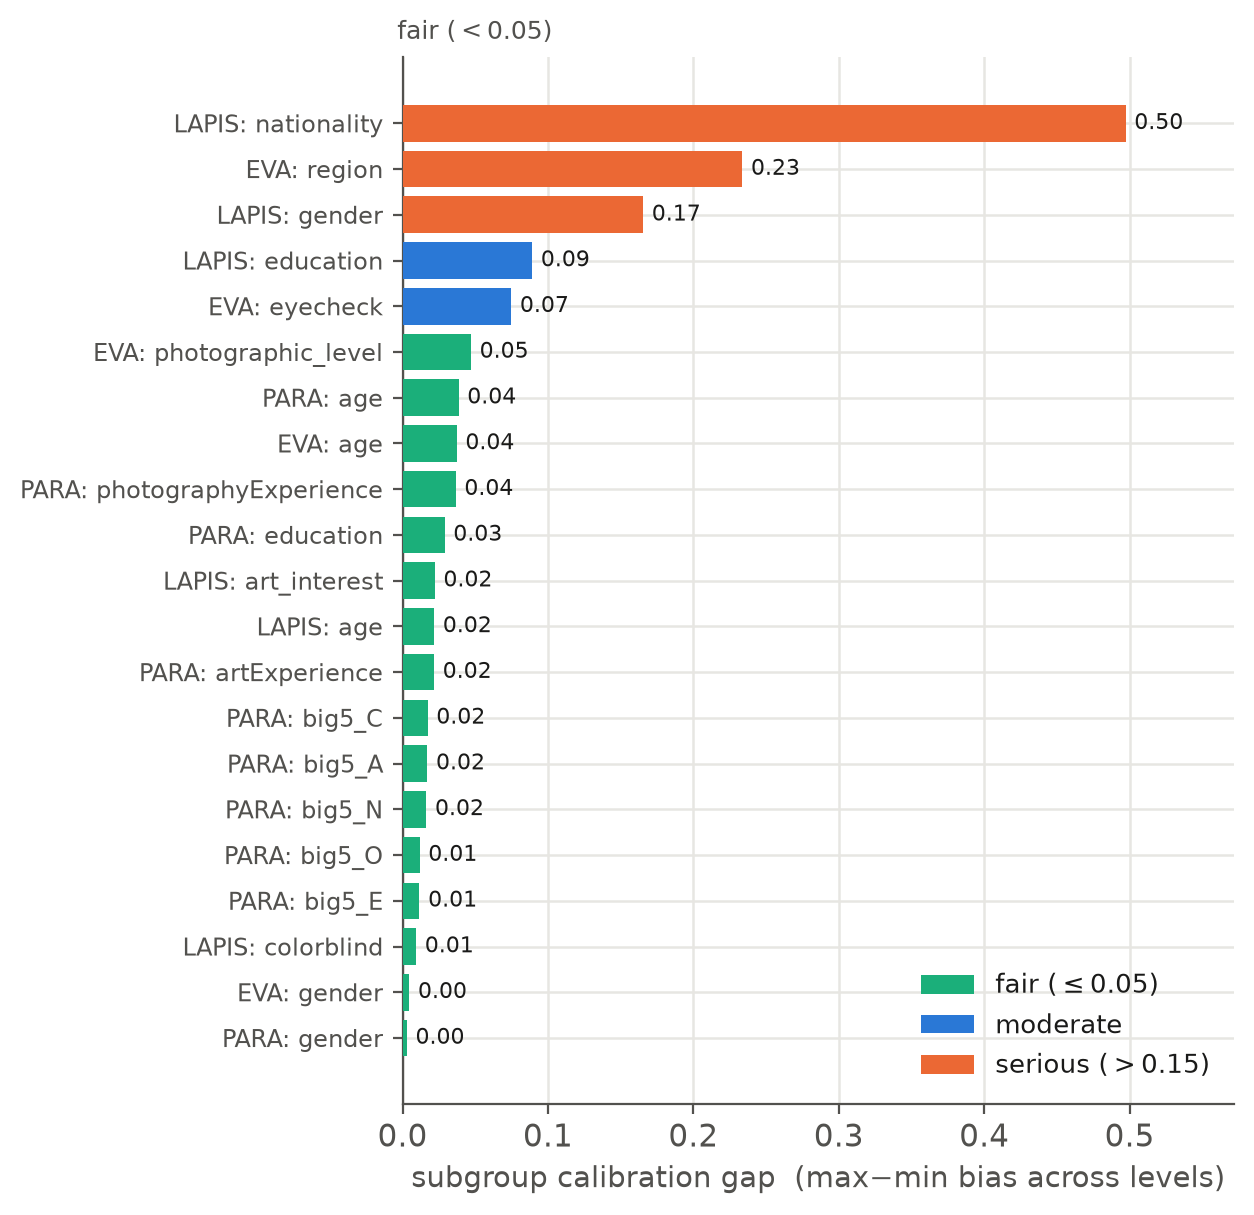
\includegraphics[width=0.72\linewidth]{figs/ax_bias.png}
  \caption{\textbf{Subgroup calibration fairness.} Calibration gap (spread of bias across a subgroup's levels) for every persona attribute, sorted. The judge is fair on most attributes but seriously biased by nationality (0.50), region (0.23), and LAPIS gender (0.17); these are flagged and controlled for rather than passed along.}
  \label{fig:bias}
\end{figure}

\section{Where the judge struggles: content categories}
Error is not uniform across content (Figure~\ref{fig:cat}): night scenes are by far the hardest category, while animals, buildings, and still life are easiest. This is a difficulty pattern, not a leakage or persona artifact, and it matches human intuition about which images are hardest to judge from a single glance.

\begin{figure}[h]
  \centering
  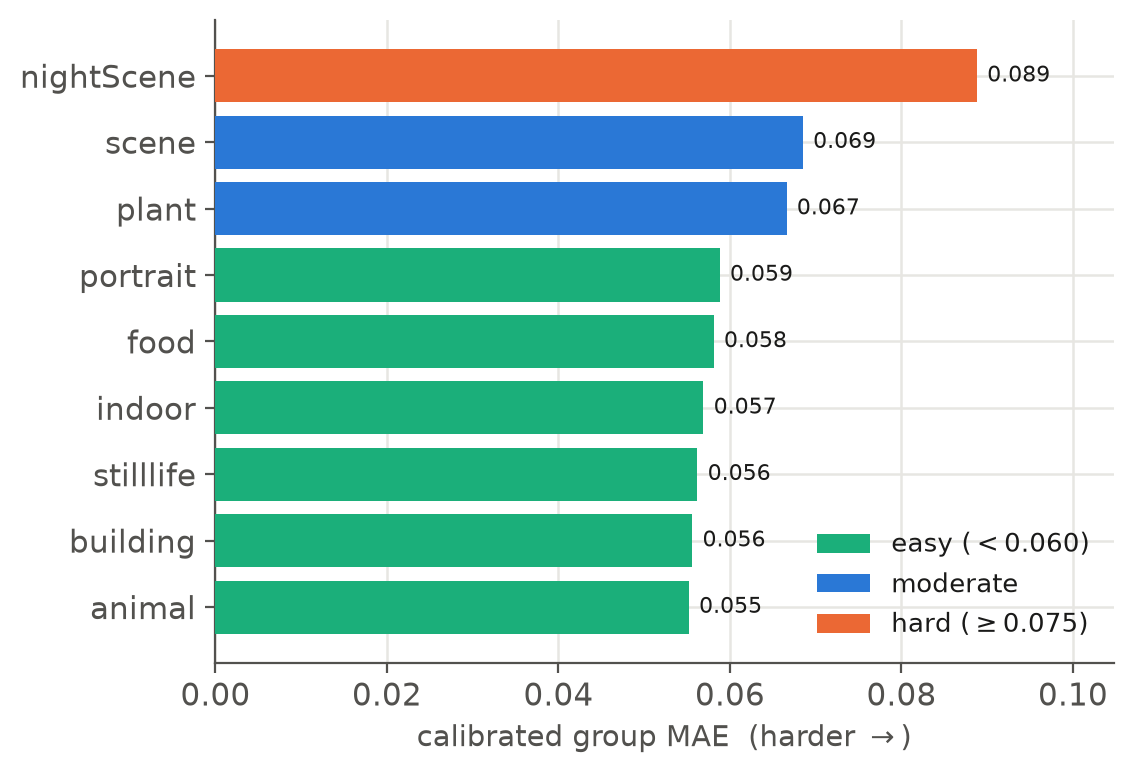
\includegraphics[width=0.6\linewidth]{figs/ax_content_category.png}
  \caption{\textbf{Difficulty by content category (PARA).} Calibrated group error per content category. Night scenes are markedly harder than the rest; the ordering is a content-difficulty effect, consistent across raters.}
  \label{fig:cat}
\end{figure}

\section{AutoPolish dynamics: convergence and identity}
Figure~\ref{fig:c4quant} in the main text shows how the refinement loop behaves over its ten steps and where the committed edits land relative to the identity guardrail: all conditions rise and saturate by step 3-4, the reward-only oracle traces the ceiling, and the three critic conditions overlap on this generic objective, the measurement ceiling discussed there. Figure~\ref{fig:c4head} restates the per-condition mean gain as bars with bootstrap intervals, and adds the same gain-versus-identity scatter at full size.

\begin{figure}[h]
  \centering
  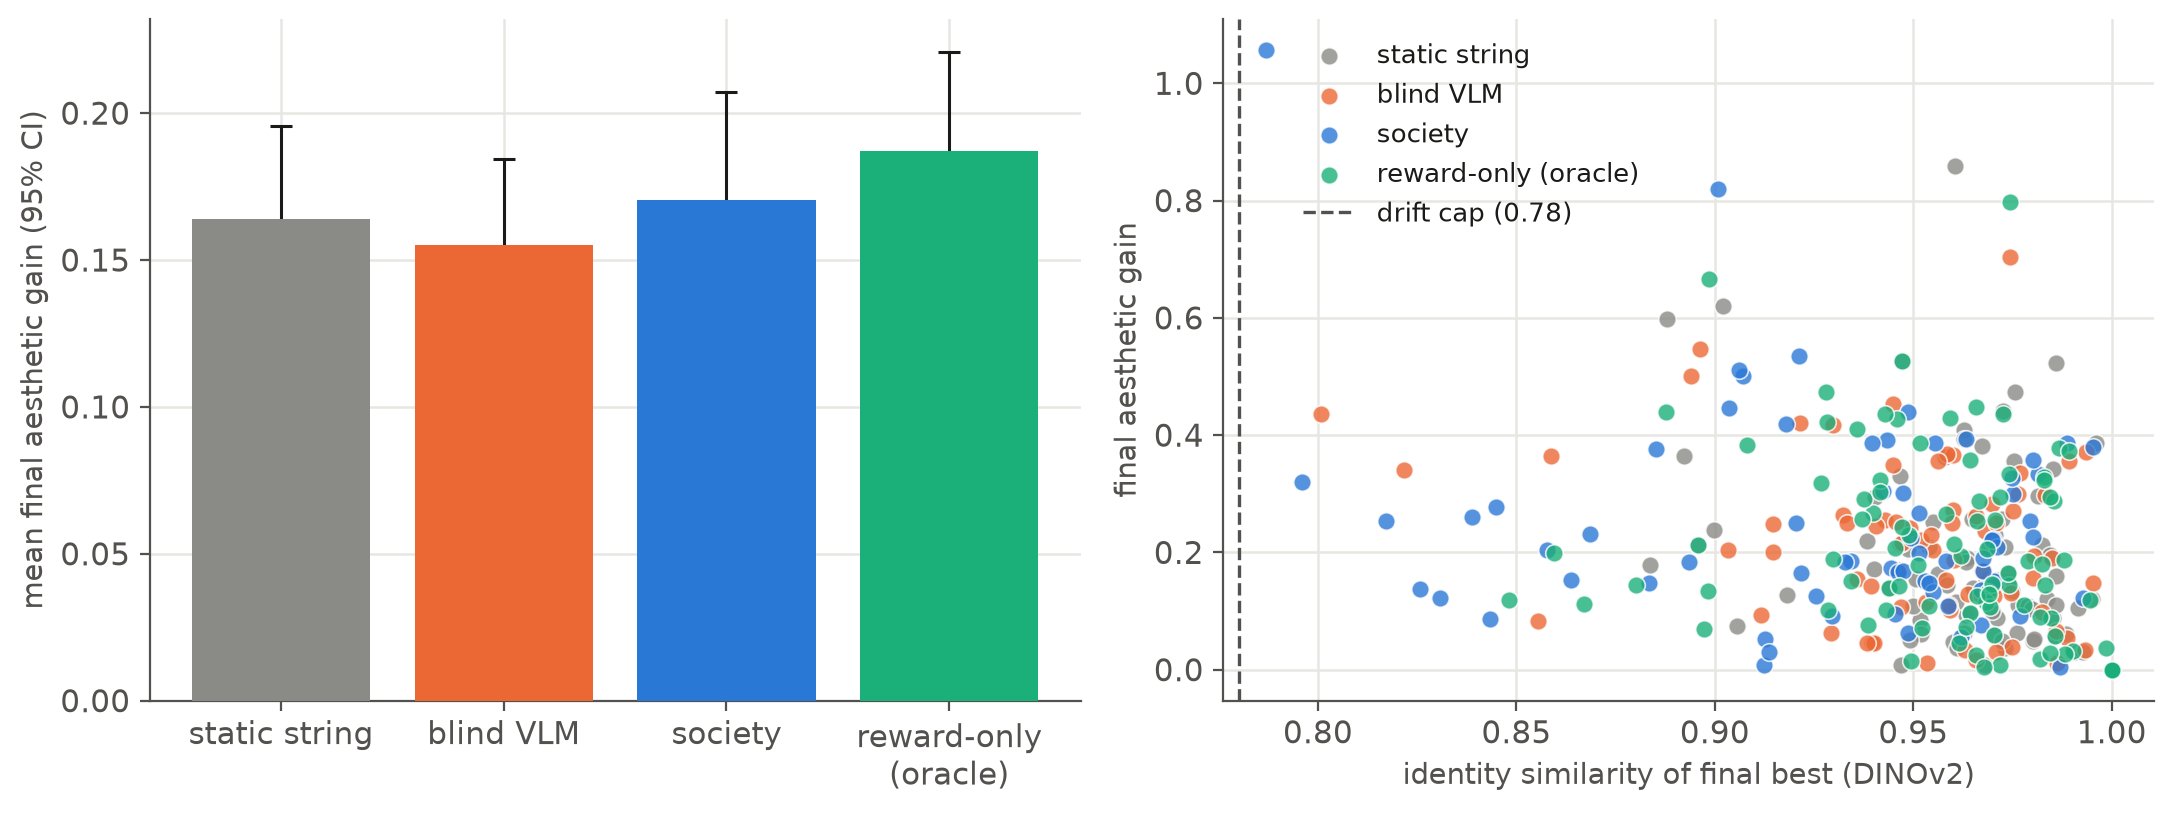
\includegraphics[width=0.98\linewidth]{figs/c4_headline.png}
  \caption{\textbf{AutoPolish gains per condition.} Left: mean final held-out aesthetic gain; every interval excludes zero. Right: each committed final image plotted by gain against DINOv2 identity similarity, with the 0.78 drift cap marked.}
  \label{fig:c4head}
\end{figure}

\section{Additional qualitative AutoPolish results}
Figure~\ref{fig:c4-qual-full} shows the complete top-five grid from which the main paper's figure takes its second and third rows, and Figure~\ref{fig:c4-qual2} a further set of images restricted to cases where the society critic attains the highest held-out score. As before, the audience critic proposes semantically meaningful changes that the fixed string and the generic critic do not: adding a player behind a basketball, revealing a kitchen behind a chef, opening a bright sky behind a structure, adding a vehicle to an empty snowy courtyard, and intensifying a sunset.

\begin{figure}[h]
  \centering
  
\includegraphics[width=0.86\linewidth]{figs/c4_qualitative.png}
  \caption{\textbf{Complete top-five qualitative grid.} Source versus best edit per condition, with held-out aesthetic scores, for the five images with the largest society-minus-static gain.}
  \label{fig:c4-qual-full}
\end{figure}

\begin{figure}[h]
  \centering
  \includegraphics[width=0.92\linewidth]{figs/ax_qualitative2.png}
  \caption{\textbf{Additional qualitative AutoPolish results.} Source versus best edit per condition, with held-out aesthetic scores, for a further set of high society-gain images. The audience critic (\textsc{society}) makes the largest, most semantically meaningful improvements and achieves the top score on every row.}
  \label{fig:c4-qual2}
\end{figure}

\section{The refinement loop over time}
Figure~\ref{fig:c4-prog} visualizes the auto-research loop itself, at full size and for all eight images (the main text lifts two of these rows into Figure~\ref{fig:c4prog}): each row is one image, and the columns are the best-so-far result after refinement steps $0, 2, 4, 6$, and $10$. Read left to right, each row shows the image being progressively polished as the audience critic accumulates and applies its complaints, with the held-out aesthetic score rising monotonically along the way. The edits are visible and semantically coherent over time: a Milky Way emerging over a night road, a sunset road gaining light and a passing vehicle, a wildlife scene brightening into focus.

\begin{figure}[h]
  \centering
  \includegraphics[width=0.92\linewidth]{figs/ax_progression.png}
  \caption{\textbf{The AutoPolish loop over time.} For the society critic, the best-so-far image after refinement steps $0, 2, 4, 6, 10$ (columns), one image per row. The held-out aesthetic score rises monotonically across steps by construction, and the visible edits accumulate coherently rather than in a single jump.}
  \label{fig:c4-prog}
\end{figure}

\section{Robustness and validity checks}
Table~\ref{tab:robust} collects the remaining sanity checks. There is no memorization signal, the group result is invariant to how duplicate ratings are handled, the judge is more accurate exactly where human raters agree, its self-reported difficulty tracks real human disagreement, and it reproduces the human inter-dimension correlation structure. Together these support that the group signal is genuine rather than an artifact of leakage or bookkeeping.

\begin{table}[h]
  \caption{Robustness and validity checks. Every diagnostic points the ``valid'' way: no memorization, invariance to duplicate handling, higher accuracy where raters agree, a valid difficulty signal, and preserved cross-dimension structure.}
  \label{tab:robust}
  \centering
  \small
  \setlength{\tabcolsep}{4pt}
  \begin{tabularx}{\linewidth}{@{}
      >{\raggedright\arraybackslash\hsize=0.85\hsize}X
      >{\raggedright\arraybackslash\hsize=1.30\hsize}X
      >{\raggedright\arraybackslash\hsize=0.85\hsize}X @{}}
    \toprule
    Check & Statistic & Reading \\
    \midrule
    Memorization (LAPIS) & Spearman(artist rating-volume, error) $=+0.03$ & no fame effect: no leakage \\
    Style difficulty (LAPIS) & best$\to$worst style MAE gap $=0.04$ & Minimalism hardest: difficulty, not leakage \\
    Duplicate ratings (LAPIS) & group MAE $=0.072$ under all 3 handlings & invariant to duplicate bookkeeping \\
    Predictability vs agreement (LAPIS) & corr(disagreement, group error) $=-0.19$ & more accurate where raters agree \\
    Difficulty validity (EVA) & corr(VLM difficulty, human disagreement) $=+0.14$ & difficulty signal is valid \\
    Cross-dimension structure (EVA) & structure-match corr $=0.77$ & reproduces the human axis correlations \\
    \bottomrule
  \end{tabularx}
\end{table}



\section{Limitations and honest negatives}
\label{sec:limits}

We report our negatives in full; each sharpens the claim and points to a next experiment. \textbf{(1) The panel-size curve is flat on real images.} Greedy decoding collapses the panel and temperature-0.7 did not fix it: the backbone reverts to the mode about 88\% of the time on discrete rating tasks. The mechanism is nonetheless clean on generated images and every separation is identical across temperatures, so the headline is no artifact; the fix, reading the token-level score distribution in one forward pass, is designed and parked. \textbf{(2) Cross-cultural differentiation on generated images is null,} under-powered at roughly one vote per cell and limited to a single generator pairing; a powered re-run with a persona-blind control is specified. \textbf{(3) The critic ablation is null on a generic objective,} which cannot resolve audience-specific critique quality; a group-preference evaluator is the fix. \textbf{(4) Thin personas break persona claims,} as EVA shows throughout. \textbf{(5) The judge carries a national rating bias.} A subgroup audit \citep{aesbiasbench2025} finds it fair across personality, age, gender, and expertise (gaps at most 0.04) but biased by nationality (0.50) and region (0.23), an ethics headline and a confound, which is why the generated-image analysis carries global-preference and persona-blind controls that net it out. Leakage, by contrast, is clean: artist fame correlates with error at only $+0.03$, the parse rate is $\approx$100\%, and the zero-shot pipeline uses no AVA exemplars, so the EVA-in-AVA overlap opens no leakage path. None undercuts the core claims: the ceiling, between-group recovery on paintings, aggregation transfer, and the validated AutoPolish loop.


\section{Future directions}
\label{sup:future}
Three extensions follow directly from the results above. Each preserves the distinction that organizes the paper, that the group is learnable and the individual is not, and each is stated as a falsifiable test rather than an aspiration.

\paragraph{Across model families and sizes: is the audience a property of the method or of one backbone?} Every number in this paper comes from a single frozen judge, \texttt{Qwen2-VL-7B-Instruct}. That establishes the mechanism exists; it does not establish that it belongs to persona-conditioned aggregation rather than to one model's idiosyncrasies. The clean experiment holds everything else fixed (persona cards, prompts, calibration protocol, folds, seeds, bootstrap) and swaps only the judge, sweeping both \emph{families} (a second open multimodal family, and a hosted frozen model as an upper reference) and \emph{sizes} within one family, so that family and capacity are separable rather than confounded. Three predictions make the sweep falsifiable. First, the persona-richness ordering LAPIS $>$ PARA $>$ EVA should survive every backbone, because it is a property of how richly the datasets describe their viewers and not of the model reading those descriptions; a backbone that reorders it would mean our richness explanation is wrong. Second, between-group separation should rise with scale and instruction-following, since the persona has to be both attended to and expressible in the output. Third, the central-tendency bias should change in magnitude but not vanish, which would confirm that post-hoc calibration is a structural prerequisite of prompted rating rather than a patch for one model. A valuable secondary readout is whether any backbone dissolves limitation~(1) of Section~\ref{sec:limits}: the flat panel-size curve on real images comes from greedy decoding reverting to the modal score about 88\% of the time, so a backbone with a genuinely broader score distribution, or the token-level score readout we describe there, would give aggregation the spread it needs to show itself on real images as it already does on generated ones. If the ordering holds and the panel-size curves rise across families, the synthetic audience is a property of the method; if it holds only for Qwen, the honest conclusion is a backbone effect, and we would report it as one.

\paragraph{Beyond images: audio, text, and mixed panels.} Nothing in the method is specifically visual. A modality needs only three ingredients to carry the pipeline: a corpus of stimuli rated by \emph{identifiable} annotators, so persona cards are built from real attributes and whole users can be held out cold-start; a frozen model that accepts that modality; and, for the editing loop, a held-out grader from a different model family plus an editor that can be anchored to the original artifact. For \textbf{audio}, music and sound-aesthetics corpora with per-listener metadata supply the first ingredient: the panel reacts to a clip, aggregation predicts the listener group's response, and the AutoPolish analogue distills the panel's complaints into one mixing or arrangement instruction applied to the original take, graded by a held-out audio-preference model with a similarity check standing in for the identity constraint. For \textbf{text}, stories and essays with annotator demographics play the same role, with a rewriter as the editor and a held-out preference model as the grader; here the identity constraint becomes semantic: the revision must not change what the piece says. In each case the first study to run is the ceiling analysis rather than the headline: ICC(1) against ICC($k$), and the persona-$\Delta R^2$, say before any modeling whether a group signal exists and how much of the individual is reachable at all. We expect the qualitative pattern to repeat, with individuals near noise and group means reliable, and the persona-richness dependence to bind harder in text, where a reader's background plausibly explains more of the variance than it does for a photograph. A further step is \emph{mixed panels}, where a persona reacts to an image with its caption or a video with its soundtrack; the open question is whether group agreement rises when a modality is added, or whether each added channel supplies one more thing for viewers to disagree about.

\paragraph{Beyond frozen: per-persona adaptation with LoRA.} Keeping every model frozen is what makes this method cheap, reproducible, and non-circular, but it also caps how much of a viewer can be represented: the persona reaches the model only as text in the context window. The natural next step moves part of the persona into \emph{parameters}, fitting a low-rank adapter \citep{hu2022lora} on the frozen backbone so that a viewer's behavior is learned rather than prompted. The design question is what one adapter should stand for, and our own ceiling result answers it. With ICC(1) between 0.19 and 0.47 and a prompted persona effect worth only 1-4\% of individual $R^2$, an adapter fit to a single annotator would mostly fit noise. The better unit is a \emph{bank of attribute adapters}, one per persona attribute or attribute cluster (art expertise, high openness, a nationality group), composed at inference into whichever card the panel calls for. This keeps the training set per adapter large, preserves the compositional structure of the cards, and, unlike a per-user model, targets exactly the level at which the signal was shown to live. The evaluation must be the same three-part one used here: individual-level $R^2$ against both the 1-4\% prompted baseline and the ICC(1) ceiling; between-group separation against the persona-blind control; and whether the isotonic calibration map still transfers across datasets, which is the property a trained model is most likely to break. Two hazards deserve stating in advance. \textbf{Leakage:} an adapter trained on the rating pool it is evaluated on would void the cold-start claim, so user-disjoint and image-disjoint folds stop being a control and become a requirement. \textbf{Circularity:} a learned critic sits closer in distribution to the objective it optimizes against, so the critic $\neq$ objective separation that makes AutoPolish credible would have to be re-measured rather than inherited. The honest framing is a trade. Adaptation buys fidelity to individuals at the price of the frozen claim, and it is worth paying only if it lifts individual-level prediction appreciably above what prompting already reaches, which the ceiling analysis says is a narrow target, and which is precisely why it is worth measuring.


%%%%%%%%%%%%%%%%%%%%%%%%%%%%%%%%%%%%%%%%%%%%%%%%%%%%%%%%%%%%
% ---- Prompts and worked examples (end of supplement) ----
%%%%%%%%%%%%%%%%%%%%%%%%%%%%%%%%%%%%%%%%%%%%%%%%%%%%%%%%%%%%

\section{Prompts}
\label{sup:prompts}
Every judgment comes from a frozen VLM under one of the system/user prompt pairs below; no weights are trained. The persona judge (the synthetic audience) and the persona-blind control differ only in the framing shown here. Inside the editing loop, a distiller prompt turns the panel's accumulated complaints into a single imperative instruction.

\paragraph{Persona judge (synthetic audience).} The free-text persona card is inserted verbatim at \pt{\{description\}}.
\begin{promptbox}{System prompt}
\ttfamily\footnotesize
You are role-playing as a person described as follows: \{description\}\\[4pt]
You are shown an image, as if it appeared in your social media feed. React the way this specific person actually would: let their personality, background, values, and taste -- not generic politeness -- decide whether they love it, are indifferent, or dislike it. Not everything deserves a high score; be honest and critical when the image doesn't match this person's taste. Do not mention that you are an AI or that you are role-playing.
\end{promptbox}
\begin{promptbox}{User prompt}
\ttfamily\footnotesize
As this exact person, look at this image. Give it an overall aesthetic score from 0 to 100 for how much YOU personally like it, then name the SINGLE change that would most improve it for your taste. Respond with ONLY a JSON object and nothing else, in exactly this form:\\[2pt]
\{"score": <integer 0-100>, "comment": "<one concrete improvement, imperative>"\}
\end{promptbox}

\paragraph{Persona-blind control (the baseline to beat).}
\begin{promptbox}{System prompt}
\ttfamily\footnotesize
You are an impartial, general-purpose judge of photographic aesthetics.\\[4pt]
You are shown one photograph. Judge it on its own merits the way a typical viewer would, without adopting any particular person's perspective or taste. Not every photo deserves a good score; be honest when a photo is mediocre or disappointing. Do not mention that you are an AI.
\end{promptbox}
\begin{promptbox}{User prompt}
\ttfamily\footnotesize
Look at this image. Give it an overall aesthetic score from 0 to 100, then name the SINGLE most important change that would most improve it. Respond with ONLY a JSON object and nothing else, in exactly this form:\\[2pt]
\{"score": <integer 0-100>, "comment": "<one concrete improvement, imperative>"\}
\end{promptbox}

\paragraph{Distiller (complaints $\to$ one edit instruction).} The running instruction is fed back so complaints accumulate across steps.
\begin{promptbox}{System prompt}
\ttfamily\footnotesize
You are a photo-editing assistant. You convert viewer feedback into ONE concrete, imperative image-edit instruction. Output only the instruction -- no preamble, no quotes, no explanation.
\end{promptbox}
\begin{promptbox}{User prompt}
\ttfamily\footnotesize
[The current edit instruction is: "<accumulated>".]\\[2pt]
Viewers looking at this image want these changes:\\
- <complaint 1>\\
- <complaint 2>\\
\ \ \dots\\[2pt]
Rewrite everything into ONE concrete imperative photo-edit instruction of at most 15 words that an image editor can apply. Output only the instruction.
\end{promptbox}

\section{Example: a panel reacting to one image}
\label{sup:panel-example}
To make the synthetic audience concrete, Figure~\ref{fig:ex-edit} (left) shows one office photograph (an open-plan office, initial held-out aesthetic 5.57), and the boxes below give five of the ten panelists' \emph{actual} reactions to it, produced by the persona prompt above (each panelist returns a score out of 100 and the single change they would most want). The panel does not agree on one thing: the two older, less art-experienced panelists ask for warmer, more natural lighting, while the others ask for plants or artwork to personalize the desks.

\begin{personabox}{Panelist~1: male, 26 to 29, senior high school, art: competent \quad(score 60/100)}
\small ``The lighting could be more natural to make the space feel more inviting.''
\end{personabox}
\begin{personabox}{Panelist~5: male, 35 to 40, senior high school, art: expert \quad(score 60/100)}
\small ``The lighting could be more natural to enhance the warmth and comfort of the space.''
\end{personabox}
\begin{personabox}{Panelist~3: female, 30 to 34, university, art: proficient \quad(score 60/100)}
\small ``Add some plants or artwork to the desks to add some life and personality to the space.''
\end{personabox}
\begin{personabox}{Panelist~6: male, 35 to 40, junior college, art: beginner \quad(score 60/100)}
\small ``Add some plants or artwork to the desks to make the space feel more welcoming and lively.''
\end{personabox}
\begin{personabox}{Panelist~9: female, 18 to 21, junior college, art: beginner \quad(score 60/100)}
\small ``Add some plants or artwork to the desks to make the space feel more welcoming and personal.''
\end{personabox}

\section{Example: from panel feedback to an edit instruction}
\label{sup:aggregation}
The loop collects the panel's ten complaints, distills them into one imperative instruction with the distiller prompt above, applies it to the \emph{original} image with the editor, and commits the result only if the held-out judge improves. For the office image the panel's two themes, lighting and personalization, are merged into a single instruction, and the committed edit adds warmer light, potted plants, and framed artwork, raising the held-out aesthetic from 5.57 to 5.96 (Figure~\ref{fig:ex-edit}).

\begin{instrbox}{Aggregated panel complaints (10 panelists)}
\small
$\bullet$~more natural, warmer lighting to make the space inviting \hfill (2 panelists)\\
$\bullet$~add plants or artwork to the desks to add life and personality \hfill (8 panelists)
\end{instrbox}
\begin{instrbox}{Distilled edit instruction ($\leq 15$ words)}
\small\itshape
Add natural lighting and plants/artwork to the desks to enhance warmth, comfort, and personalization.
\end{instrbox}

\begin{figure}[h]
  \centering
  \begin{subfigure}{0.42\linewidth}\centering
    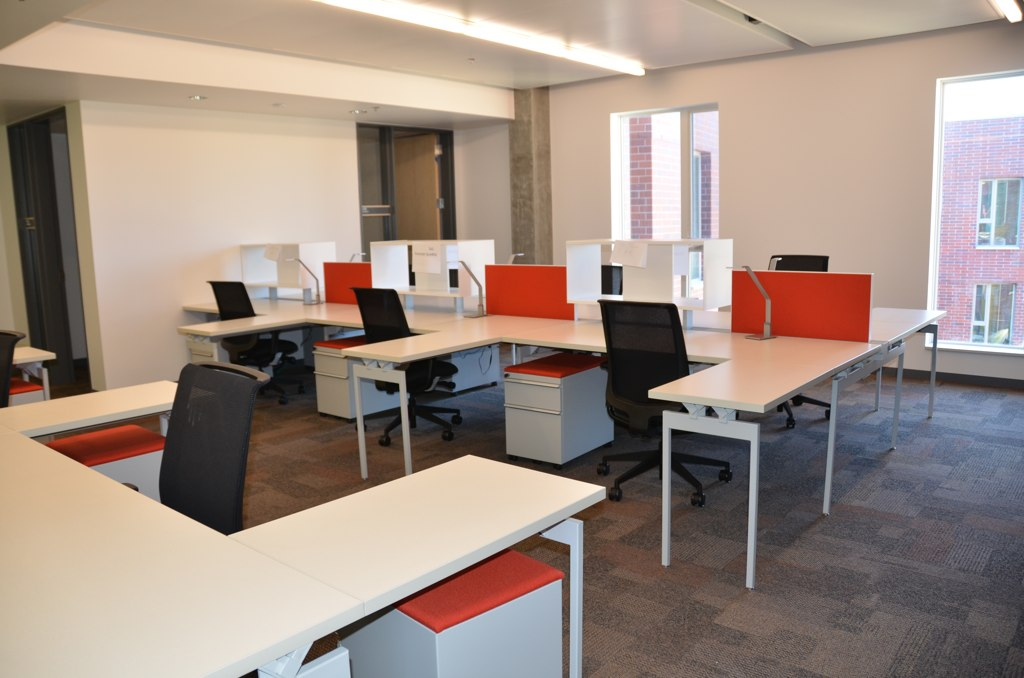
\includegraphics[width=\linewidth]{figs/ex_office_src.jpg}\caption{source (aes 5.57)}\end{subfigure}\hspace{0.04\linewidth}
  \begin{subfigure}{0.42\linewidth}\centering
    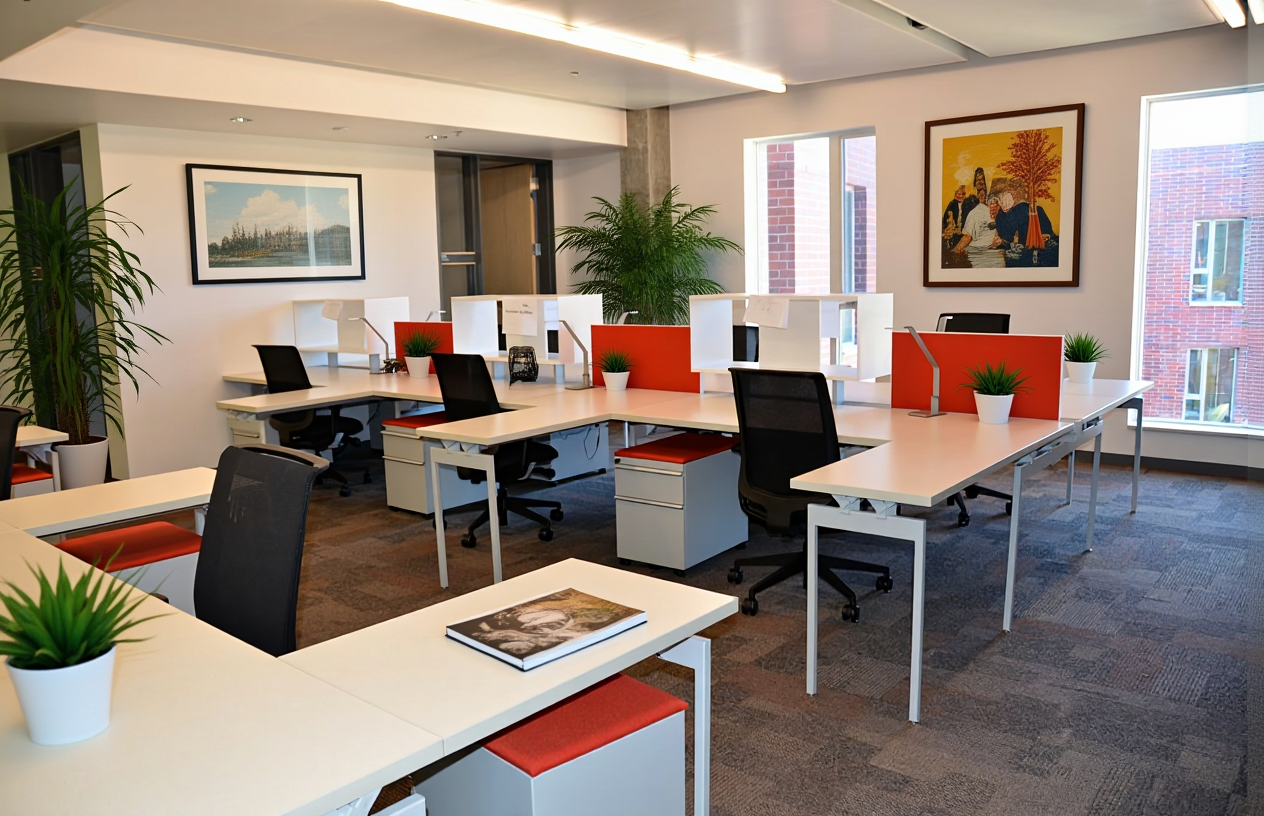
\includegraphics[width=\linewidth]{figs/ex_office_edit.png}\caption{after one step (aes 5.96)}\end{subfigure}
  \caption{\textbf{From complaints to a committed edit.} Left: the office source (held-out aesthetic 5.57) that the panel in Section~\ref{sup:panel-example} reacted to. Right: the audience-guided edit adds plants and framed artwork and warms the lighting, exactly the changes the panel asked for, raising the held-out aesthetic to 5.96 as confirmed by the held-out judge.}
  \label{fig:ex-edit}
\end{figure}


\end{document}
